\documentclass[letterpaper,11pt,onesided]{book}%

% After compiling the full document, compile with, for example:
%
% pdflatex -jobname=section1-6 "\includeonly{1.6-quantification3}\documentclass[12pt,oneside]{book}

\usepackage[scale=2]{ccicons}
\usepackage{caption}
\usepackage[labelfont={}]{subcaption}
\captionsetup{subrefformat=parens}
\usepackage{booktabs}
\usepackage{epigraph}
\usepackage{enumitem}
\usepackage{newclude}
\usepackage{multicol}
\usepackage{tabu}
\usepackage[table]{xcolor}
\usepackage{tikz}
\usetikzlibrary{arrows,automata,positioning,fit,shapes}
\usepackage{rotating}
\usepackage[notextcomp]{kpfonts} 
\usepackage{graphicx}
\usepackage{eurosym}
\usepackage{amsfonts}
\usepackage{amsmath}
\usepackage{amssymb}
\usepackage{stmaryrd}
\usepackage{wasysym}
\usepackage{amsthm}
\usepackage[margin=1in]{geometry}
\usepackage[hang,flushmargin]{footmisc}
\usepackage{color}
\definecolor{darkblue}{rgb}{0, 0, .6}
\definecolor{grey}{rgb}{.7, .7, .7}
\usepackage[breaklinks]{hyperref}
\hypersetup{
	colorlinks=true,
	linkcolor=darkblue,
	anchorcolor=darkblue,
	citecolor=darkblue,
	pagecolor=darkblue,
	urlcolor=darkblue,
	pdftitle={},
	pdfauthor={},
    bookmarksnumbered
}

\usepackage{fancyhdr}
\pagestyle{fancy}
\lhead{\leftmark}
\chead{}
\rhead{}
\lfoot{}
\cfoot{\thepage}
\rfoot{}

\theoremstyle{definition}
\newtheorem{theorem}{Theorem}[chapter]
\newtheorem{acknowledgement}[theorem]{Acknowledgement}
\newtheorem{algorithm}[theorem]{Algorithm}
\newtheorem{axiom}[theorem]{Axiom}
\newtheorem{case}[theorem]{Case}
\newtheorem{claim}[theorem]{Claim}
\newtheorem{conclusion}[theorem]{Conclusion}
\newtheorem{condition}[theorem]{Condition}
\newtheorem{conjecture}[theorem]{Conjecture}
\newtheorem{corollary}[theorem]{Corollary}
\newtheorem{criterion}[theorem]{Criterion}
\newtheorem{definition}[theorem]{Definition}
\newtheorem{example}[theorem]{Example}
\newtheorem{exercise}[theorem]{Exercise}
\newtheorem{journal}[theorem]{Journal}
\newtheorem{lemma}[theorem]{Lemma}
\newtheorem{notation}[theorem]{Notation}
\newtheorem{problem}[theorem]{Problem}
\newtheorem{proposition}[theorem]{Proposition}
\newtheorem{remark}[theorem]{Remark}
\newtheorem{solution}[theorem]{Solution}
\newtheorem{summary}[theorem]{Summary}
\newtheorem{skeleton}[theorem]{Skeleton Proof}
\newtheorem{activity}[theorem]{Activity}
\newtheorem{intuitivedef}[theorem]{Intuitive Definition}
\newtheorem{question}[theorem]{Question}

\newsavebox{\savepar}
\newenvironment{textbox}{\noindent\begin{lrbox}{\savepar}\begin{minipage}[c]{.98\textwidth}}{\end{minipage}\end{lrbox}\fcolorbox{black}{white}{\usebox{\savepar}}}

\newcommand{\dom}{\operatorname{Dom}}
\newcommand{\codom}{\operatorname{Codom}}
\newcommand{\range}{\operatorname{Rng}}
\newcommand{\lcm}{\operatorname{lcm}}
\newcommand{\card}{\operatorname{card}}
\newcommand{\rel}{\operatorname{rel}}
\newcommand{\Rel}{\operatorname{Rel}}

\begin{document}

\title{An Introduction to Proof via \\Inquiry-Based Learning}
\author{Dana C.~Ernst, PhD\\
Northern Arizona University}
\date{Version Spring 2021}

\maketitle
\thispagestyle{empty}

\noindent\copyright{ \the\year\ Dana C.~Ernst.  Some Rights Reserved.\\

\bigskip

\noindent This book is intended to be a task sequence for an introduction to proof course that utilizes an inquiry-based learning (IBL) approach.  You can find the most up-to-date version of these notes on GitHub:
\begin{center}
\url{http://dcernst.github.io/IBL-IntroToProof/}
\end{center}
I would be thrilled if you used these notes and improved them. If you make any modifications, you can either make a pull request on GitHub or submit the improvements via email.  You are also welcome to fork the source and modify the notes for your purposes as long as you maintain the license below.

\bigskip

\noindent This work is licensed under the Creative Commons Attribution-Share Alike 4.0 United States License.  You may copy, distribute, display, and perform this copyrighted work, but only if you give credit to Dana C.~Ernst, and all derivative works based upon it must be published under the Creative Commons Attribution-Share Alike 4.0 International License. Please attribute this work to Dana C.~Ernst, Mathematics Faculty at Northern Arizona University, \url{dana.ernst@nau.edu}, as well as the individuals listed below. To view a copy of this license, visit
\begin{center}
\url{https://creativecommons.org/licenses/by-sa/4.0/}
\end{center}
or send a letter to Creative Commons, 171 Second Street, Suite 300, San Francisco, California, 94105, USA.}

\medskip

\begin{center}
\ccbysa
\end{center}

\bigskip

\noindent Below is a partial list of people (alphabetical by last name) that I need to thank for supplying content, advice, and feedback.
\begin{itemize}
\item \href{https://thalestriangles.blogspot.com}{Joshua Bowman} (Pepperdine University). The Preface is a modified version of Joshua's \emph{An IBL preface}.
\item \href{http://www.paulellis.org}{Paul Ellis} (Manhattanville College). Paul has provided lots of useful feedback and several suggestions for improvements. Paul suggested problems for Chapter~\ref{chap:Induction} and provided an initial draft of Section~\ref{sec:Images and Inverse Images}: Images and Inverse Images.
\item \href{http://jasongrout.org}{Jason Grout} (Bloomberg, L.P.).  I'm extremely grateful to Jason for feedback on early versions of this material, as well as helping me with a variety of technical aspects of writing these notes.
\item \href{http://home.snc.edu/andershendrickson/}{Anders Hendrickson} (St.~Norbert College). Anders is the original author of the content in Appendix~\ref{appendix:elements_of_style}: Elements of Style for Proofs. The current version in Appendix~\ref{appendix:elements_of_style} is a result of modifications made by myself with some suggestions from David Richeson.
\item \href{http://www.hsc.edu/rebecca-jayne}{Rebecca Jayne} (Hampden--Sydney College). The current version of Section~\ref{sec:CompleteInduction}: Complete Induction is a derivative of content contributed by Rebecca.
\item \href{http://www4.csudh.edu/library/info/civic-directory/f-j/matthew-g-jones}{Matthew Jones} (CSU Dominguez Hills) and \href{http://www.stanyoshinobu.com}{Stan Yoshinobu} (Cal Poly). A few of the sections were originally adaptations of notes written by Matt and Stan. Early versions of these notes relied heavily on their work. Moreover, Matt and Stan were two of the key players that contributed to shaping my approach to teaching.
\item \href{http://math.depaul.edu/tpeter21/}{T.~Kyle Petersen} (DePaul University) and \href{http://math.depaul.edu/bridget/}{Bridget Tenner} (DePaul University). Modifications that Kyle and Bridget made to the book inspired me to streamline some of the exposition, especially in the early chapters.
\item \href{http://users.dickinson.edu/~richesod/}{David Richeson} (Dickinson College). David is responsible for much of the content in Appendix~\ref{appendix:fancy_math_terms}: Fancy Mathematical Terms and Appendix~\ref{appendix:definitions}: Definitions in Mathematics. In addition, the current version of Chapter~\ref{chap:three famous theorems}: Three Famous Theorems is heavily based on content contributed by David.
\item \href{http://www2.kenyon.edu/Depts/Math/schumacherc/public_html/}{Carol Schumacher} (Kenyon College). When I was transitioning to an IBL approach to teaching, Carol was one of my mentors and played a significant role in my development as a teacher.  Moreover, this work is undoubtably influenced my Carol's excellent book \emph{Chapter Zero: Fundamental Notions of Advanced Mathematics}, which I used when teaching my very first IBL course.
\item \href{http://webpages.csus.edu/wiscons/}{Josh Wiscons} (CSU Sacramento). Josh contributed the content in Section~\ref{sec:ModularArithmetic}: Modular Arithmetic.
\end{itemize}

\tableofcontents
%\thispagestyle{empty}

\chapter*{Preface}
\addcontentsline{toc}{chapter}{\protect\numberline{}Preface}

%shorter
This book is intended to be used for a one-semester introduction to proof course. The book is designed around an inquiry-based learning (IBL) approach to teaching and learning mathematics, but makes no assumptions about the specifics of how the instructor chooses to implement this approach.  Loosely speaking, IBL is a student-centered method of teaching that engages students in sense-making activities.  Students are given tasks requiring them to solve problems, conjecture, experiment, explore, create, and communicate.  Rather than showing facts or a clear, smooth path to a solution, the instructor guides and mentors students via well-crafted problems through an adventure in mathematical discovery. The book includes more content than one can expect to cover in a single semester. This allows the instructor to pick and choose the sections that suit their needs and desires. Each chapter takes a focused approach to the included topics, but also includes many gentle exercises aimed at developing intuition.


%longer
This book is intended to be used for a one-semester/quarter introduction to proof course (sometimes referred to as a transition to proof course). The intended audience is mathematics majors and minors. The book is designed around an inquiry-based learning (IBL) approach to teaching and learning mathematics, but makes no assumptions about the specifics of how the instructor chooses to implement this approach.  Loosely speaking, IBL is a student-centered method of teaching that engages students in sense-making activities.  Students are given tasks requiring them to solve problems, conjecture, experiment, explore, create, and communicate.  Rather than showing facts or a clear, smooth path to a solution, the instructor guides and mentors students via well-crafted problems through an adventure in mathematical discovery.  According to \href{https://www.colorado.edu/eer/sites/default/files/attached-files/laursenrasmussencommentaryauthorversion0219.pdf}{Laursen and Rasmussen (2019)}, the Four Pillars of IBL are:
\begin{itemize}
\item Students engage deeply with coherent and meaningful mathematical tasks.
\item Students collaboratively process mathematical ideas.
\item Instructors inquire into student thinking.
\item Instructors foster equity in their design and facilitation choices.
\end{itemize}

The book includes more content than one can expect to cover in a single semester. This allows the instructor to pick and choose the sections that suit their needs and desires. Each chapter takes a focused approach to the included topics, but also includes many gentle exercises aimed at developing intuition.

%%%%%%%%%

You are the creators. This book is a guide.

This book will not show you how to solve all the problems that are presented, but it should \emph{enable} you to find solutions, on your own and working together. The material you are about to study did not come together fully formed at a single moment in history. It was composed gradually over the course of centuries, with various mathematicians building on the work of others, improving the subject while increasing its breadth and depth.

Mathematics is essentially a human endeavor. Whatever you may believe about the true nature of mathematics---does it exist eternally in a transcendent Platonic realm, or is it contingent upon our shared human consciousness?---our \emph{experience} of mathematics is temporal, personal, and communal. Like music, mathematics that is encountered only as symbols on a page remains inert. Like music, mathematics must be created in the moment, and it takes time and practice to master each piece. The creation of mathematics takes place in writing, in conversations, in explanations, and most profoundly in the mental construction of its edifices on the basis of reason and observation.

To continue the musical analogy, you might think of this textbook like a performer's score. Much is included to direct you towards particular ideas, but much is missing that can only be supplied by you: participation in the creative process that will make those ideas come alive. Moreover, your success will depend on the pursuit of both \emph{individual} excellence and \emph{collective} achievement. Like a musician in an orchestra, you should bring your best work and be prepared to blend it with others' contributions.

In any act of creation, there must be room for experimentation, and thus allowance for mistakes, even failure. A key goal of our community is that we support each other---sharpening each other's thinking but also bolstering each other's confidence---so that we can make failure a \emph{productive} experience. Mistakes are inevitable, and they should not be an obstacle to further progress. It's normal to struggle and be confused as you work through new material. Accepting that means you can keep working even while feeling stuck, until you overcome and reach even greater accomplishments.

This book is a guide. You are the creators.
\chapter{Introduction}\label{chap:intro}
%\thispagestyle{empty}

\begin{section}{What is This Course All About?}%new title?

The foundations of mathematics refers to logic and set theory; the axioms of number and space.  Also, it refers to an introduction to the techniques of proof, and at a larger level the process of \emph{doing Mathematics}.  Proof is central to doing mathematics.

Up to this point, it is likely that your experience of mathematics has been about using formulas and algorithms. That is only one part of mathematics. Mathematicians do much more than just use formulas.  Mathematicians experiment, make conjectures, write definitions, and prove theorems.  In this class, then, we will learn about doing all of these things.

What will this class require?  Daily practice.  Just like learning to play an instrument or sport, you will have to learn new skills and ideas.  Sometimes you'll feel good, sometimes frustrated.  You'll probably go through a range of feelings from being exhilarated, to being stuck.  Figuring it out, victories, defeats, and all that is part of real life is what you can expect.  Most importantly it will be rewarding.  Learning mathematics requires dedication.  It will require that you be patient despite periods of confusion.  It will require that you persevere in order to understand.  As the instructor, I am here to guide you, but I cannot do the learning for you, just as a music teacher cannot move your fingers and your heart for you.  Only you can do that.  I can give suggestions, structure the course to assist you, and try to help you figure out how to think through things.  Do your best, be prepared to put in a lot of time, and do all the work.  Ask questions in class, ask questions in office hours, and ask your classmates questions.  When you work hard and you come to understand, you feel good about yourself.  In the meantime, you have to believe that your work will pay off in intellectual development.

How will this class be organized?  You have probably heard that mathematics is not a spectator sport.  Our focus in this class is on learning to DO mathematics, not learning to sit patiently while others do it.  Therefore, class time will be devoted to working on problems, and especially on students presenting conjectures and proofs to the class, asking questions of presenters in order to understand their work and their thinking, and sharing and clarifying our thinking and understanding of each other's ideas.  

The class is fueled by your ability to prove theorems and share your ideas.  As we progress, you will find that you have ideas for proofs, but you are unsure of them.  In that case, you can either bring your idea to the class, or you can bring it to office hours.  By coming to office hours, you have a chance to refine your ideas and get individual feedback before bringing them to the class.  The more you use office hours, the more you will learn.  If the whole class is stuck, we can work on some ego-booster problems to get your ideas flowing.

Finally, this is a very exciting time in your mathematical career.  It's where you learn what mathematics is really about!

\epigraph{The mathematician does not study pure mathematics because it is useful; he studies it because he delights in it, and he delights in it because it is beautiful.}{\emph{Henri Poincar\'e}}

\end{section}

\begin{section}{An Inquiry-Based Approach}

This is not a lecture-oriented class or one in which mimicking prefabricated examples will lead you to success. You will be expected to work actively to construct your own understanding of the topics at hand with the readily available help of me and your classmates. Many of the concepts you learn and problems you work on will be new to you and ask you to stretch your thinking. You will experience \emph{frustration} and \emph{failure} before you experience \emph{understanding}. This is part of the normal learning process. If you are doing things well, you should be confused at different points in the semester. The material is too rich for a human being to completely understand it immediately. Your viability as a professional in the modern workforce depends on your ability to embrace this learning process and make it work for you.

\epigraph{Don't fear failure.  Not failure, but low aim, is the crime. In great attempts it is glorious even to fail.}{\emph{Bruce Lee}}

In order to promote a more active participation in your learning, we will incorporate ideas from an educational philosophy called inquiry-based learning (IBL).  Loosely speaking, IBL is a student-centered method of teaching mathematics that engages students in sense-making activities.  Students are given tasks requiring them to solve problems, conjecture, experiment, explore, create, and communicate.  Rather than showing facts or a clear, smooth path to a solution, the instructor guides and mentors students via well-crafted problems through an adventure in mathematical discovery.  According to \href{https://www.colorado.edu/eer/sites/default/files/attached-files/laursenrasmussencommentaryauthorversion0219.pdf}{Laursen and Rasmussen (2019)}, the Four Pillars of IBL are:
\begin{itemize}
\item Students engage deeply with coherent and meaningful mathematical tasks.
\item Students collaboratively process mathematical ideas.
\item Instructors inquire into student thinking.
\item Instructors foster equity in their design and facilitation choices.
\end{itemize}

Much of the course will be devoted to students presenting their proposed solutions or proofs on the board and a significant portion of your grade will be determined by how much mathematics you produce.  I use the word \emph{produce} because I believe that the best way to learn mathematics is by doing mathematics.  Someone cannot master a musical instrument or a martial art by simply watching, and in a similar fashion, you cannot master mathematics by simply watching; you must do mathematics!

In any act of creation, there must be room for experimentation, and thus allowance for mistakes, even failure. A key goal of our community is that we support each other---sharpening each other's thinking but also bolstering each other's confidence---so that we can make failure a productive experience. Mistakes are inevitable, and they should not be an obstacle to further progress. It's normal to struggle and be confused as you work through new material. Accepting that means you can keep working even while feeling stuck, until you overcome and reach even greater accomplishments.

\epigraph{You will become clever through your mistakes.}{\emph{German Proverb}}

Furthermore, it is important to understand that solving genuine problems is difficult and takes time.  You shouldn't expect to complete each problem in 10 minutes or less.  Sometimes, you might have to stare at the problem for an hour before even understanding how to get started.

In this course, everyone will be required to
\begin{itemize}
\item read and interact with course notes and textbook on your own;
\item write up quality solutions/proofs to assigned problems;
\item present solutions/proofs on the board to the rest of the class;
\item participate in discussions centered around a student's presented solution/proof;
\item call upon your own prodigious mental faculties to respond in flexible, thoughtful, and creative ways to problems that may seem unfamiliar on first glance.
\end{itemize}
As the semester progresses, it should become clear to you what the expectations are.

\epigraph{Tell me and I forget, teach me and I may remember, involve me and I learn.}{\emph{Benjamin Franklin}}

\end{section}

\begin{section}{Rights of the Learner}
As a student in this class, you have the right:
\begin{enumerate}
\item to be confused,
\item to make a mistake and to revise your thinking,
\item to speak, listen, and be heard, and
\item to enjoy doing mathematics.
\end{enumerate}

\epigraph{You may encounter many defeats, but you must not be defeated.}{\emph{Maya Angelou}}
	
\end{section}

\begin{section}{Your Toolbox, Questions, and Observations}

Throughout the semester, we will develop a list of \emph{tools} that will help you understand and do mathematics. Your job is to keep a list of these tools, and it is suggested that you keep a running list someplace.

Next, it is of utmost importance that you work to understand every proof. (Every!)  Questions are often your best tool for determining whether you understand a proof.  Therefore, here are some sample questions that apply to any proof that you should be prepared to ask of yourself or the presenter:
\begin{itemize}
\item What method(s) of proof are you using?
\item What form will the conclusion take?
\item How did you know to set up that [equation, set, whatever]?
\item How did you figure out what the problem was asking?
\item Was this the first thing you tried?
\item Can you explain how you went from this line to the next one?
\item What were you thinking when you introduced this?
\item Could we have \ldots instead?
\item Would it be possible to \ldots?
\item What if \ldots?
\end{itemize}

Another way to help you process and understand proofs is to try and make observations and connections between different ideas, proof statements and methods, and to compare approaches used by different people. Observations might sound like some of the following:
\begin{itemize}
\item When I tried this proof, I thought I needed to \ldots But I didn't need that, because \ldots
\item I think that \ldots is important to this proof, because \ldots
\item When I read the statement of this theorem, it seemed similar to this earlier theorem. Now I see that it [is/isn't] because \ldots
\end{itemize}

\end{section}

\begin{section}{Rules of the Game}
You should \emph{not} look to resources outside the context of this course for help. That is, you should not be consulting the Internet, other texts, other faculty, or students outside of our course. On the other hand, you may use each other, the course notes, me, and your own intuition.  In this class, earnest failure outweighs counterfeit success; you need not feel pressure to hunt for solutions outside your own creative and intellectual reserves.  For more details, check out the Syllabus.

\end{section}

\begin{section}{Structure of the Notes}

As you read the notes, you will be required to digest the material in a meaningful way.  It is your responsibility to read and understand new definitions and their related concepts.  However, you will be supported in this sometimes difficult endeavor. In addition, you will be asked to complete exercises aimed at solidifying your understanding of the material.  Most importantly, you will be asked to make conjectures, produce counterexamples, and prove theorems.

Most items in the notes are labelled with a number.  The items labelled as \textbf{Definition} and \textbf{Example} are meant to be read and digested.  However, the items labelled as \textbf{Exercise}, \textbf{Question}, \textbf{Theorem}, \textbf{Corollary}, and \textbf{Problem} require action on your part.  In particular, items labelled as \textbf{Exercise} are typically computational in nature and are aimed at improving your understanding of a particular concept.  There are very few items in the notes labelled as \textbf{Question}, but in each case it should be obvious what is required of you.  Items with the \textbf{Theorem} and \textbf{Corollary} designation are mathematical facts and the intention is for you to produce a valid proof of the given statement.  The main difference between a \textbf{Theorem} and \textbf{Corollary} is that corollaries are typically statements that follow quickly from a previous theorem.  In general, you should expect corollaries to have very short proofs.  However, that doesn't mean that you can't produce a more lengthy yet valid proof of a corollary.  The items labelled as \textbf{Problem} are sort of a mixed bag.  In many circumstances, I ask you to provide a counterexample for a statement if it is false or to provide a proof if the statement is true.  Usually, I have left it to you to determine the truth value.  If the statement for a problem is true, one could relabel it as a theorem.

It is important to point out that there are very few examples in the notes.  This is intentional.  One of the goals of the items labelled as \textbf{Exercise} is for you to produce the examples.

Lastly, there are many situations where you will want to refer to an earlier definition or theorem/corollary/problem.  In this case, you should reference the statement by number.  For example, you might write something like, ``By Theorem 2.14, we see that\ldots."

\end{section}

\begin{section}{Some Minimal Guidance}
Especially in the opening sections, it won't be clear what facts from your prior experience in mathematics we are ``allowed" to use.  Unfortunately, addressing this issue is difficult and is something we will sort out along the way.  However, in general, here are some minimal and vague guidelines to keep in mind.  

First, there are times when we will need to do some basic algebraic manipulations.  You should feel free to do this whenever the need arises.  But you should show sufficient work along the way.  You do not need to write down justifications for basic algebraic manipulations (e.g., adding 1 to both sides of an equation, adding and subtracting the same amount on the same side of an equation, adding like terms, factoring, basic simplification, etc.).  

On the other hand, you do need to make explicit justification of the logical steps in a proof.  When necessary, you should cite a previous definition, theorem, etc. by number.

Unlike the experience many of you had writing proofs in geometry, our proofs will be written in complete sentences.  You should break sections of a proof into paragraphs and use proper grammar.  There are some pedantic conventions for doing this that I will point out along the way.  Initially, this will be an issue that most students will struggle with, but after a few weeks everyone will get the hang of it.

Ideally, you should rewrite the statements of theorems before you start the proof.  Moreover, for your sake and mine, you should label the statement with the appropriate number.  I will expect you to indicate where the proof begins by writing ``\emph{Proof.}" at the beginning.  Also, we will conclude our proofs with the standard ``proof box" (i.e., $\square$ or $\blacksquare$), which is typically right-justified.

Lastly, every time you write a proof, you need to make sure that you are making your assumptions crystal clear.  Sometimes there will be some implicit assumptions that we can omit, but at least in the beginning, you should get in the habit of stating your assumptions up front.  Typically, these statements will start off ``Assume\ldots" or ``Let\ldots".  

This should get you started.  We will discuss more as the semester progresses.  Now, go have fun and start exploring mathematics!

\epigraph{If you want to sharpen a sword, you have to remove a little metal.}{\emph{Unknown}}

\end{section}
\include*{IntroToMath}
\include*{TasteNumberTheory}
\include*{IntroToLogic}
\include*{NegatingAndContradiction}
\include*{IntroQuantification}
\include*{MoreQuantification}
\include*{IntroSetTheoryTopology}
\include*{Sets}
\include*{RussellsParadox}
\include*{PowerSets}
\include*{IndexingSets}
\include*{Topology}
\include*{Induction}
\include*{IntroInduction}
\include*{MoreInduction}
\include*{CompleteInduction}
\include*{ThreeFamousTheorems}
\include*{FundamentalTheoremArithmetic}
\include*{IrrationalityRoot2}
\include*{InfinitudeOfPrimes}
\include*{RelationsPartitions}
\include*{CartesianProducts}
\include*{Relations}
\include*{EquivalenceRelations}
\include*{Partitions}
\include*{ModularArithmetic}
%\include*{Posets}
\include*{Functions}
\include*{IntroFunctions}
\include*{ImagesInverseImages}
\include*{CompositionsInverses}
\include*{Cardinality}
\include*{IntroCardinality}
\include*{FiniteSets}
\include*{InfiniteSets}
\include*{CountableSets}
\include*{UncountableSets}
%\include*{OrderRelations}
%Appendices
\appendix
\chapter{Elements of Style for Proofs}
\label{appendix:elements_of_style}

Mathematics is about discovering proofs and writing them clearly and compellingly. The following guidelines apply whenever you write a proof.  Keep these guidelines handy so that you may refer to them as you write your proofs.

\begin{enumerate}

\item \textbf{The burden of communication lies on you, not on your reader.}
It is your job to explain your thoughts; it is not your reader's job to guess them from a few hints. You are trying to convince a skeptical reader who does not believe you, so you need to argue with airtight logic in crystal clear language; otherwise the reader will continue to doubt. If you did not write something on the paper, then (a) you did not communicate it,(b) the reader did not learn it, and (c) the grader has to assume you did not know it in the first place.
          
\item \textbf{Tell the reader what you are proving or citing.}
The reader does not necessarily know or remember what ``Theorem 2.13'' is. Even a professor grading a stack of papers might lose track from time to time. Therefore, the statement you are proving should be on the same page as the beginning of your proof. 

In most proofs you will want to refer to an earlier definition, problem, theorem, or corollary.  In this case, you should reference the statement by number, but it is also helpful to the reader to summarize the statement you are citing.  For example, you might write something like, ``By Theorem~2.3, the sum of two consecutive integers is odd, and so\ldots."

\item \textbf{Use English words.}
Although there will usually be equations or mathematical statements in your proofs, use English sentences to connect them and display their logical relationships. If you look at proofs in textbooks and research papers, you will see that they consist mostly of English words.

\item \textbf{Use complete sentences.}
If you wrote a history essay in sentence fragments, the reader would not understand what you meant; likewise in mathematics you must use complete sentences, with verbs, to convey your logical train of thought.
        
Some complete sentences can be written purely in mathematical symbols, such as equations (e.g., $a^3=b^{-1}$), inequalities (e.g., $x<5$), and other relations (like $5\big|10$ or $7\in\mathbb{Z}$). These statements usually express a relationship between two mathematical \emph{objects}, like numbers or sets.  However, it is considered bad style to begin a sentence with symbols.  A common phrase to use to avoid starting a sentence with mathematical symbols is ``We see that...''.

\item \textbf{Show the logical connections among your sentences.}
Use phrases like ``Therefore'', ``Thus", ``Hence", ``Then", ``since", ``because'', ``if\ldots, then\ldots'', or ``if and only if'' to connect your sentences.
  
\item \textbf{Know the difference between statements and objects.}
A mathematical object is a \emph{thing}, a noun, such as a set, an element, a number, an ordered pair, a vector space, etc. Objects either exist or do not exist. Statements, on the other hand, are mathematical \emph{sentences}:  they are either true or false.
        
When you see or write a cluster of math symbols, be sure you know whether it is an object (e.g., ``$x^2+3$'') or a statement (e.g., ``$x^2+3<7$''). One way to tell is that every mathematical statement includes a verb, such as $=$, $\leq$, $\in$, ``divides'', etc.
        
\item \textbf{The symbol ``$=$'' means ``equals".}
Do not write $A=B$ unless you mean that $A$ actually equals $B$. This guideline seems obvious, but there is a great temptation to be sloppy.  In calculus, for example, some people might write $f(x)=x^{2}=2x$ (which is false), when they really mean that ``if $f(x)=x^{2}$, then $f'(x)=2x$.''

\item \textbf{Do not interchange ${=}$ and ${\implies}$.}
The equals sign connects two \emph{objects}, as in ``$x^2=b$''; the symbol ``$\implies$'' is an abbreviation for ``implies'' and connects two \emph{statements}, as in ``$a+b=a \implies b=0$.''  You should avoid using $\implies$ in formal write-ups of proofs.

\item \textbf{Avoid logical symbols in your proofs.}  
Similar to $\implies$, you should avoid using the logical symbols $\forall, \exists, \vee, \wedge$, and $\logeq$ in your formal write-ups.  These symbols are useful for abbreviating in your scratch work. 

\item \textbf{Say exactly what you mean.}
Just as $=$ is sometimes abused, so too people sometimes write $A\in B$ when they mean $A\subseteq B$, or write $a_{ij}\in A$ when they mean that $a_{ij}$ is an entry in matrix $A$. Mathematics is a very precise language, and there is a way to say exactly what you mean; find it and use it.

\item \textbf{Do not utilize anything unproven.}
Every statement in your proof should be something you \emph{know} to be true. The reader expects your proof to be a series of statements, each proven by the statements that came before it. If you ever need to write something you do not yet know is true, you \emph{must} preface it with words like ``assume,'' ``suppose,'' or ``if'' if you are temporarily assuming it, or with words like ``we need to show that'' or ``we claim that'' if it is your goal. Otherwise, the reader will think they have missed part of your proof.

\item \textbf{Write strings of equalities (or inequalities) in the proper order.}
When your reader sees something like
\[
A=B\leq C=D,
\]
they expect to understand easily why $A=B$, why $B\leq C$, and why $C=D$, and they expect the point of the entire line to be the more complicated fact that $A\leq D$. For example, if you were computing the distance $d$ of the point $(12,5)$ from the origin, you could write
\[
d = \sqrt{12^2+5^2} = 13.
\]
In this string of equalities, the first equals sign is true by the Pythagorean theorem, the second is just arithmetic, and the conclusion is that the first item equals the last item: $d=13$.
        
A common error is to write strings of equations in the wrong order. For example, if you were to write ``$\sqrt{12^2+5^2}=13=d$'', your reader would understand the first equals sign, would be baffled as to how we know $d=13$, and would be utterly perplexed as to why you wanted or needed to go through $13$ to prove that $\sqrt{12^2+5^2}=d$.

\item \textbf{Avoid circularity.}  Be sure that no step in your proof makes use of the conclusion!
        
\item \textbf{Do not write the proof backwards.}
Beginning students often attempt to write ``proofs'' like the following, which attempts to prove that $\tan^2(x)  = \sec^2(x) - 1$:
\begin{align*}
\tan^2(x) & = \sec^2(x) - 1 \\
\left(\frac{\sin(x)}{\cos(x)}\right)^2 & = \frac{1}{\cos^2(x)} - 1 \\
\frac{\sin^2(x)}{\cos^2(x)} & =  \frac{1-\cos^2(x)}{\cos^2(x)} \\
\sin^2(x) & = 1-\cos^2(x) \\
\sin^2(x) + \cos^2(x) & = 1 \\
1 & = 1
\end{align*}        
Notice what has happened here:  the student \emph{started} with the conclusion, and deduced the true statement ``$1=1$.'' In other words, they have proved ``If $\tan^2(x) = \sec^2(x) - 1$, then $1=1$,'' which is true but highly uninteresting.
        
Now this is not a bad way of \emph{finding} a proof. Working backwards from your goal often is a good strategy \emph{on your scratch paper}, but when it is time to \emph{write} your proof, you have to start with the hypotheses and work to the conclusion.

Here is an example of a suitable proof for the desired result, where each expression follows from the one immediately proceeding it:
\begin{align*}
\sec^2(x) - 1 & = \frac{1}{\cos^2(x)} - 1\\
& = \frac{1-\cos^2(x)}{\cos^2(x)} \\
& = \frac{\sin^2(x)}{\cos^2(x)} \\
& = \left(\frac{\sin(x)}{\cos(x)}\right)^2 \\
& = \left(\tan(x)\right)^2 \\
& = \tan^2(x).
\end{align*}

\item \textbf{Be concise.}
Many beginning proof writers err by writing their proofs too short, so that the reader cannot understand their logic. It is nevertheless quite possible to be too wordy, and if you find yourself writing a full-page essay, it is possible that you do not really have a proof, but just some intuition. When you find a way to turn that intuition into a formal proof, it will be much shorter.

\item \textbf{Introduce every symbol you use.}
If you use the letter ``$k$,'' the reader should know exactly what $k$ is. Good phrases for introducing symbols include ``Let $n\in \mathbb{N}$,'' ``Let $k$ be the least integer such that\ldots,'' ``For every real number $a$\ldots,'' and ``Suppose $A\subseteq\mathbb{R}\ldots$".
          
\item \textbf{Use appropriate quantifiers (once).}
When you introduce a variable $x\in S$, it must be clear to your reader whether you mean ``for all $x\in S$'' or just ``for some $x\in S$.'' If you just say something like ``$y=x^2$ where $x\in S$,'' the word ``where'' does not indicate whether you mean ``for all'' or ``some''.
        
Phrases indicating the quantifier ``for all'' include ``Let $x\in S$''; ``for all $x\in S$''; ``for every $x\in S$''; ``for each $x\in S$''; etc. Phrases indicating the quantifier ``some'' or ``there exists'' include ``for some $x\in S$''; ``there exists an $x\in S$''; ``for a suitable choice of $x\in S$''; etc.

Once you have said ``Let $x\in S$,'' the letter $x$ has its meaning defined. You do not need to say ``for all $x\in S$'' again, and you definitely should \emph{not} say ``let $x\in S$'' again.

\item \textbf{Use a symbol to mean only one thing.}
Once you use the letter $x$ once, its meaning is fixed for the duration of your proof. You cannot use $x$ to mean anything else. There is an exception to this guideline.  Sometimes a proof will include multiple subproofs that are distinct from each other.  In this case, you can reuse a variable or symbol as long as it is clear to the reader that you have concluded with the previous subproof and have moved onto a new subproof.   

\item \textbf{Do not ``prove by example.''}\label{pfbyexample}
Most problems ask you to prove that something is true ``for all''---You \emph{cannot} prove this by giving a single example, or even a hundred. Your proof will need to be a logical argument that holds for \emph{every example there possibly could be}.

On the other hand, if the claim that you are trying to prove involves the existence of a mathematical object with a particular property, then providing a specific example is sufficient.
        
\item \textbf{Write ``Let $x=\dots$,'' not ``Let $\dots=x$.''} 
When you have an existing expression, say $a^{2}$, and you want to give it a new, simpler name like $b$, you should write ``Let $b=a^{2}$,'' which means, ``Let the new symbol $b$ mean $a^{2}$.'' This convention makes it clear to the reader that $b$ is the brand-new symbol and $a^{2}$ is the old expression he/she already understands.
        
If you were to write it backwards, saying ``Let $a^{2}=b$,'' then your startled reader would ask, ``What if $a^{2}\neq b$?''
  
\item \textbf{Make your counterexamples concrete and specific.}
Proofs need to be entirely general, but counterexamples should be concrete. When you provide an example or counterexample, make it as specific as possible. For a set, for example, you must specify its elements, and for a function you must specify the corresponding relation (possibly an algebraic rule) and its domain and codomain. Do not say things like ``$f$ could be one-to-one but not onto''; instead, provide an actual function $f$ that is one-to-one but not onto.
    
\item \textbf{Do not include examples in proofs.}
Including an example very rarely adds anything to your proof. If your logic is sound, then it does not need an example to back it up. If your logic is bad, a dozen examples will not help it (see Guideline~\ref{pfbyexample}). There are only two valid reasons to include an example in a proof: if it is a \emph{counterexample} disproving something, or if you are performing complicated manipulations in a general setting and the example is just to help the reader understand what you are saying.

 \item \textbf{Use scratch paper.}
Finding your proof will be a long, potentially messy process,  full of false starts and dead ends. Do all that on scratch paper until you find a real proof, and only then break out your clean paper to write your final proof carefully.
        
Only sentences that actually contribute to your proof should be part of the proof. Do not just perform a ``brain dump,'' throwing everything you know onto the paper before showing the logical steps that prove the conclusion. \emph{That is what scratch paper is for.}

\end{enumerate}
\chapter{Fancy Mathematical Terms}
\label{appendix:fancy_math_terms}

Here are some important mathematical terms that you will encounter in this course and throughout your mathematical career.

\begin{enumerate}
\item
\textbf{Definition}---a precise and unambiguous description of the meaning of a mathematical term.  It characterizes the meaning of a word by giving all the properties and only those properties that must be true.
\item
\textbf{Theorem}---a mathematical statement that is proved using rigorous mathematical reasoning.  In a mathematical paper, the term theorem is often reserved for the most important results.
\item
\textbf{Lemma}---a minor result whose sole purpose is to help in proving a theorem.  It is a stepping stone on the path to proving a theorem. Very occasionally lemmas can take on a life of their own (Zorn's Lemma, Urysohn's Lemma, Burnside's Lemma, Sperner's Lemma).
\item
\textbf{Corollary}---a result in which the (usually short) proof relies heavily on a given theorem (we often say that ``this is a corollary of Theorem A'').
\item
\textbf{Proposition}---a proved and often interesting result, but generally less important than a theorem.
\item
\textbf{Conjecture}---a statement that is unproved, but is believed to be true (Collatz Conjecture, Goldbach Conjecture, Twin prime Conjecture).
\item
\textbf{Claim}---an assertion that is then proved.  It is often used like an informal lemma.
\item
\textbf{Axiom/Postulate}---a statement that is assumed to be true without proof. These are the basic building blocks from which all theorems are proved (Euclid's five postulates, axioms of ZFC, Peano axioms).
\item
\textbf{Identity}---a mathematical expression giving the equality of two (often variable) quantities (trigonometric identities, Euler's identity).
\item
\textbf{Paradox}---a statement that can be shown, using a given set of axioms and definitions, to be both true and false. Paradoxes are often used to show the inconsistencies in a flawed axiomatic theory (e.g., Russell's Paradox).  The term paradox is also used informally to describe a surprising or counterintuitive result that follows from a given set of rules (Banach-Tarski Paradox, Alabama Paradox, Gabriel's Horn).
\end{enumerate}
\chapter{Paradoxes}
\label{appendix:paradoxes}

A \textbf{paradox} is a statement that can be shown, using a given set of axioms and definitions, to be both true and false. Recall that an axiom is a statement that is assumed to be true without proof. These are the basic building blocks from which all theorems are proved. Paradoxes are often used to show the inconsistencies in a flawed axiomatic theory.  The term paradox is also used informally to describe a surprising or counterintuitive result that follows from a given set of rules. In Section~\ref{sec:RussellsParadox}, we encountered two paradoxes:
\begin{itemize}
\item The Barber of Seville (Problem~\ref{prob:barber})
\item Russell's Paradox (Problem~\ref{prob:russell})
\end{itemize}
Below are several additional paradoxes that are worth exploring.

%The following paradoxes are from Dave Richeson.
\begin{enumerate}
\item \textbf{Librarian's Paradox.} A librarian is given the unenviable task of creating two new books for the library. Book A contains the names of all books in the library that reference themselves and Book B contains the names of all books in the library that do not reference themselves. But the librarian just created two new books for the library, so their titles must be in either Book A or Book B. Clearly Book A can be listed in Book B, but where should the librarian list Book B?

\item \textbf{Liar's Paradox.} Consider the statement: this sentence is false. Is it true or false?

\item \textbf{Berry Paradox.} Consider the claim: every natural number can be unambiguously described in fourteen words or less. It seems clear that this statement is false, but if that is so, then there is some smallest natural number which cannot be unambiguously described in fourteen words or less. Let's call it $n$. But now $n$ is ``the smallest natural number that cannot be unambiguously described in fourteen words or less.'' This is a complete and unambiguous description of $n$ in fourteen words, contradicting the fact that $n$ was supposed not to have such a description. Therefore, all natural numbers can be unambiguously described in fourteen words or less!

\item \textbf{The Naming Numbers Paradox.} Consider the claim: every natural number can be unambiguously described using no more than 50 characters (where a character is a--z, 0--9, and a ``space''). For example, we can describe 9 as ``9'' or ``nine'' or ``the square of the second prime number.'' There are only 37 characters, so we can describe at most $37^{50}$ numbers, which is very large, but not infinite. So the statement is false. However, here is a ``proof'' that it is true. Let $S$ be the set of natural numbers that can be unambiguously described using no more than 50 characters. For the sake of contradiction, suppose it is not all of $\mathbb{N}$. Then there is a smallest number $t\in\mathbb{N}\setminus S$. We can describe $t$ as: the smallest natural number not in $S$.  Thus $t$ can be described using no more than 50 characters. So $t\in S$, a contradiction.

\item \textbf{Euathlus and Protagoras.} Euathlus wanted to become a lawyer but could not pay Protagoras. Protagoras agreed to teach him under the condition that if Euathlus won his first case, he would pay Protagoras, otherwise not. Euathlus finished his course of study and did nothing. Protagoras sued for his fee. He argued:\\

\noindent If Euathlus loses this case, then he must pay (by the judgment of the court).\\
If Euathlus wins this case, then he must pay (by the terms of the contract).\\
He must either win or lose this case.\\
Therefore Euathlus must pay me.\\

\noindent But Euathlus had learned well the art of rhetoric. He responded:\\

\noindent If I win this case, I do not have to pay (by the judgment of the court).\\
If I lose this case, I do not have to pay (by the contract).\\
I must either win or lose the case.\\
Therefore, I do not have to pay Protagoras.
\end{enumerate}
\chapter{Definitions in Mathematics}
\label{appendix:definitions}
\thispagestyle{empty}

It is difficult to overstate the importance of definitions in mathematics. Definitions play a different role in mathematics than they do in everyday life. 

Suppose you give your friend a piece of paper containing the definition of the rarely-used word \textbf{rodomontade}. According to the Oxford English Dictionary\footnote{http://www.oed.com/view/Entry/166837} (OED) it is:
\begin{quote}
A vainglorious brag or boast; an extravagantly boastful, arrogant, or bombastic speech or piece of writing; an arrogant act.
\end{quote}
Give your friend some time to study the definition. Then take away the paper. Ten minutes later ask her to define rodomontade. Most likely she will be able to give a reasonably accurate definition. Maybe she'd say something like, ``It is a speech or act or piece of writing created by a pompous or egotistical person who wants to show off how great they are.'' It is unlikely that she will have quoted the OED word-for-word. In everyday English that is fine---you would probably agree that your friend knows the meaning of the rodomontade. This is because most definitions are \emph{descriptive}. They describe the common usage of a word. 

Let us take a mathematical example. The OED\footnote{http://www.oed.com/view/Entry/40280}  gives this definition of \emph{continuous}.
\begin{quote}
Characterized by continuity; extending in space without interruption of substance; having no interstices or breaks; having its parts in immediate connection; connected, unbroken.
\end{quote}
Likewise, we often hear calculus students speak of a continuous function as one whose graph can be drawn ``without picking up the pencil.'' This definition is descriptive. (As we learned in calculus the picking-up-the-pencil description is not a perfect description of continuous functions.) This is not a mathematical definition. 

Mathematical definitions are \emph{prescriptive}. The definition must prescribe the exact and correct meaning  of a word. Contrast the OED's descriptive definition of continuous with the the definition of continuous found in a real analysis textbook.
\begin{quote}
A function $f:A\to \mathbb{R}$ is \textbf{continuous at a point} $c\in A$ if,  for all $\varepsilon>0$, there exists $\delta>0$ such that whenever $|x-c|<\delta$ (and $x\in A$) it follows that $|f(x)-f(c)|<\varepsilon$. If $f$ is continuous at every point in the domain $A$, then we say that $f$ is \textbf{continuous on} $A$.\footnote{This definition is taken from page 109 of Stephen Abbott's \emph{Understanding Analysis}, but the definition would be essentially the same in any modern real analysis textbook.} 
\end{quote}
In mathematics there is very little freedom in definitions. Mathematics is a deductive theory; it is impossible to state and prove theorems without clear definitions of the mathematical terms. The definition of a term must completely, accurately, and unambiguously describe the term. Each word is chosen very carefully and the order of the words is  critical. In the definition of continuity changing ``there exists'' to ``for all,'' changing the orders of quantifiers, changing $<$ to $\leq$ or $>$, or changing $\mathbb{R}$ to $\mathbb{Z}$ would completely change the meaning of the definition. 

What does this mean for you, the student? Our recommendation is that at this stage you memorize the definitions word-for-word. It is the safest way to guarantee that you have it correct. As you gain confidence and familiarity with the subject you may be ready to modify the wording. You may want to change ``for all'' to ``given any'' or you may want to change $|x-c|<\delta$ to $-\delta<x-c<\delta$ or to ``the distance between $x$ and $c$ is less than $\delta$.'' 

Of course, memorization is not enough; you must have a conceptual understanding of the term, you must see how the formal definition matches up with your conceptual understanding, and you must know how to work with the definition. It is perhaps with the first of these that descriptive definitions are useful. They are useful for building intuition and for painting the ``big picture.'' Only after days (weeks, months, years?) of experience does one get an intuitive feel for the $\varepsilon,\delta$-definition of continuity; most mathematicians have the ``picking-up-the-pencil'' definitions in their head. This is fine as long as we know that it is imperfect, and that when we prove theorems about continuous functions in mathematics we use the mathematical definition. 

We end this discussion with an amusing real-life example in which a descriptive definition was not sufficient. In 2003 the German version of the game show \emph{Who wants to be a millionaire?} contained the following question: ``Every rectangle is: (a) a rhombus, (b) a trapezoid, (c) a square, (d) a parallelogram.'' 

The confused contestant decided to skip the question and left with \euro 4000. Afterward the show received letters from irate viewers. Why were the contestant and the viewers upset with this problem? Clearly a rectangle is a parallelogram, so (d) is the answer. But what about (b)? Is a rectangle a trapezoid? We would describe a trapezoid as a quadrilateral with a pair of parallel sides. But this leaves open the question: can a trapezoid have \emph{two} pairs of parallel sides or must there only be \emph{one} pair? The viewers said two pairs is allowed, the producers of the television show said it is not. This is a case in which a clear, precise, mathematical definition is required.

\end{document}
"
%
% to get a file with just section 1.6 in it with the correct theorem numbering, etc.


\newif\ifinstructor
%% uncomment one of the following, depending if you want to include the
%% instructor notes or not
\instructortrue
%\instructorfalse


\newif\ifnotes
%% uncomment one of the following, depending if you want to include the
%% instructor notes or not
\notestrue
%\notesfalse

\usepackage{tabls}
\usepackage{booktabs}
\usepackage{amsmath}
\usepackage{amssymb}
\usepackage{amsthm}
\usepackage{amsfonts}
\usepackage{multicol}
\usepackage{enumitem}
\usepackage{stmaryrd}
\usepackage{wasysym}
\usepackage{microtype}
\usepackage{tikz}
\usetikzlibrary{positioning,arrows,automata}
\usepackage[hang,flushmargin,symbol*]{footmisc}
\usepackage{comment}
\usepackage{graphicx}
\usepackage{wrapfig}
\usepackage{color}
\definecolor{darkblue}{rgb}{0, 0, .6}
\definecolor{grey}{rgb}{.7, .7, .7}
\usepackage[breaklinks]{hyperref}
\hypersetup{
	colorlinks=true,
	linkcolor=darkblue,
	anchorcolor=darkblue,
	citecolor=darkblue,
	pagecolor=darkblue,
	urlcolor=darkblue,
	pdftitle={},
	pdfauthor={}
}

\usepackage[margin=1in]{geometry}

%%%%%%%%%%%%%%%%%%%%%%%%%%%%%%%%%%%%%%%%%%%%%%%%%%%%%%%%%%%%%%%%%%%%%%%%%%%%%%%%%%%%%%%%%%%%%%%%%%%%%%
% Margin notes
%%%%%%%%%%%%%%%%%%%%%%%%%%%%%%%%%%%%%%%%%%%%%%%%%%%%%%%%%%%%%%%%%%%%%%%%%%%%%%%%%%%%%%%%%%%%%%%%%%%%%%
%\usepackage[left=1in,right=2.75in,top=1in,bottom=1in]{geometry}
%\marginparwidth 1.75in
%\let\oldmarginpar\marginpar
%\renewcommand\marginpar[1]{\-\oldmarginpar{\raggedright\footnotesize #1}}
%\renewcommand\marginpar[1]{\-\oldmarginpar[\raggedleft\footnotesize #1]{\raggedright\footnotesize #1}}




%%%%%%%%%%%%%%%%%%%%%%%%%%%%%%%%%%%%%%%%%%%%%%%%%%%%%%%%%%%%%%%%%%%%%%%%%%%%%%%%%%%%%%%%%%%%%%%%%%%%%%
% Embed the date and time into every page
%%%%%%%%%%%%%%%%%%%%%%%%%%%%%%%%%%%%%%%%%%%%%%%%%%%%%%%%%%%%%%%%%%%%%%%%%%%%%%%%%%%%%%%%%%%%%%%%%%%%%%
%\usepackage[12hr]{datetime}
%\newdateformat{draftdate}{%
%\shortdayofweekname{\THEDAY}{\THEMONTH}{\THEYEAR}, %
%\THEDAY\ \shortmonthname[\THEMONTH] \THEYEAR}
%\draftdate
%\usepackage{eso-pic}
%\AddToShipoutPicture{\put(10,10){\small Draft: \today\ at \currenttime }}%--- version: \MakeUppercase{\svnInfoRevision}}}

%%%%%%%%%%%%%%%%%%%%%%%%%%%%%%%%%%%%%%%%%%%%%%%%%%%%%%%%%%%%%%%%%%%%%%%%%%%%%%%%%%%%%%%%%%%%%%%%%%%%%%
% Instructor-specific material (answers, helps, etc.)
%%%%%%%%%%%%%%%%%%%%%%%%%%%%%%%%%%%%%%%%%%%%%%%%%%%%%%%%%%%%%%%%%%%%%%%%%%%%%%%%%%%%%%%%%%%%%%%%%%%%%%
\ifinstructor
  \newcommand{\instructor}[1]{\marginpar{\textbf{Instructor: }#1}}
\else
  \newcommand{\instructor}[1]{}
\fi

%%%%%%%%%%%%%%%%%%%%%%%%%%%%%%%%%%%%%%%%%%%%%%%%%%%%%%%%%%%%%%%%%%%%%%%%%%%%%%%%%%%%%%%%%%%%%%%%%%%%%%
% Personal notes about improving the text, etc.
%%%%%%%%%%%%%%%%%%%%%%%%%%%%%%%%%%%%%%%%%%%%%%%%%%%%%%%%%%%%%%%%%%%%%%%%%%%%%%%%%%%%%%%%%%%%%%%%%%%%%%
\ifnotes
\renewcommand{\thefootnote}{\roman{footnote}}
\newcommand{\note}[1]{\footnote{#1}\marginpar{\fbox{\textbf{\thefootnote}}}}
\else
\newcommand{\note}[1]{}
\fi



%%%%%%%%%%%%%%%%%%%%%%%%%%%%%%%%%%%%%%%%%%%%%%%%%%%%%%%%%%%%%%%%%%%%%%%%%%%%%%%%%%%%%%%%%%%%%%%%%%%%%%
% Commands to define a term (so that we get nice indexing
%%%%%%%%%%%%%%%%%%%%%%%%%%%%%%%%%%%%%%%%%%%%%%%%%%%%%%%%%%%%%%%%%%%%%%%%%%%%%%%%%%%%%%%%%%%%%%%%%%%%%%
\newcommand{\define}[2][]{\textbf{#2}\index{#1#2}}
\newcommand{\definemargin}[2][]{\marginpar{#2}\define[#1]{#2}}

%%%%%%%%%%%%%%%%%%%%%%%%%%%%%%%%%%%%%%%%%%%%%%%%%%%%%%%%%%%%%%%%%%%%%%%%%%%%%%%%%%%%%%%%%%%%%%%%%%%%%%
% Theorems
%%%%%%%%%%%%%%%%%%%%%%%%%%%%%%%%%%%%%%%%%%%%%%%%%%%%%%%%%%%%%%%%%%%%%%%%%%%%%%%%%%%%%%%%%%%%%%%%%%%%%%

\newtheoremstyle{box}%
{}{}% standard spacing before and after
{}% Body style
{}{\bfseries}{.}% Heading indent, font, and punctuation
{ }% space after heading
{\thmname{#1}\thmnumber{ #2}\thmnote{: #3}}% head spec

\newtheoremstyle{problem}%
{}{}% standard spacing before and after
{}% Body style
{}{\bfseries}{}% Heading indent, font, and punctuation
{1em}% space after heading
{\fbox{\thmname{#1}\thmnumber{ #2}}\thmnote{ (#3)}}% head spec


\theoremstyle{problem}
\newtheorem{theorem}{Theorem}[chapter]
\newtheorem{question}[theorem]{Question}
\newtheorem{problem}[theorem]{Problem}
\newtheorem{exercise}[theorem]{Exercise}
\newtheorem{corollary}[theorem]{Corollary}
\newtheorem{conjecture}[theorem]{Conjecture}
\newtheorem{lemma}[theorem]{Lemma}

\theoremstyle{definition}
\newtheorem{theorem-given}{Theorem}[chapter]
\newtheorem{lemma-given}[theorem]{Lemma}
\newtheorem{acknowledgement}[theorem]{Acknowledgement}
\newtheorem{algorithm}[theorem]{Algorithm}
\newtheorem{axiom}[theorem]{Axiom}
\newtheorem{case}[theorem]{Case}
\newtheorem{claim}[theorem]{Claim}
\newtheorem{conclusion}[theorem]{Conclusion}
\newtheorem{condition}[theorem]{Condition}
\newtheorem{criterion}[theorem]{Criterion}
\newtheorem{definition}[theorem]{Definition}
\newtheorem{example}[theorem]{Example}
\newtheorem{journal}[theorem]{Journal}
\newtheorem{notation}[theorem]{Notation}
\newtheorem{proposition}[theorem]{Proposition}
\newtheorem{remark}[theorem]{Remark}
\newtheorem{solution}[theorem]{Solution}
\newtheorem{summary}[theorem]{Summary}
\newtheorem{skeleton}[theorem]{Skeleton Proof}


\newsavebox{\savepar}
\newenvironment{textbox}{\noindent\begin{lrbox}{\savepar}\begin{minipage}[c]{.98\textwidth}}{\end{minipage}\end{lrbox}\fcolorbox{black}{white}{\usebox{\savepar}}}
\newenvironment{section*}[1]{\section*{#1}}{}


%%%%%%%%%%%%%%%%%%%%%%%%%%%%%%%%%%%%%%%%%%%%%%%%%%%%%%%%%%%%%%%%%%%%%%%%%%%%%%%%%%%%%%%%%%%%%%%%%%%%%%
% Notation shortcuts
%%%%%%%%%%%%%%%%%%%%%%%%%%%%%%%%%%%%%%%%%%%%%%%%%%%%%%%%%%%%%%%%%%%%%%%%%%%%%%%%%%%%%%%%%%%%%%%%%%%%%%

\DeclareMathOperator{\dom}{Dom}
\DeclareMathOperator{\codom}{Codom}
\DeclareMathOperator{\range}{Rng}
\newcommand{\blank}[1]{\raisebox{0pt}[14pt]{\rule{#1}{0.7pt}}}

\let\origdoublepage\cleardoublepage

\newcommand{\clearemptydoublepage}{%
  \clearpage
  {\pagestyle{empty}\origdoublepage}%
}



\begin{document}
\frontmatter


\title{Course Notes for Introduction to Proof}
\author{D.C.~Ernst\thanks{Northern Arizona University, \url{Dana.Ernst@nau.edu}}}
\date{Typeset on \today\\
\vfill
  Part of this work is an adaptation of notes written by Stan Yoshinobu of Cal Poly and Matthew Jones of California State University, Dominguez Hills.
\vfill

\includegraphics[height=1.3cm]{by-sa}
\vfill}
\maketitle
 \thispagestyle{empty}

\noindent\copyright{ 2013 Dana Ernst, Stan Yoshinobu, Matthew Jones.  Some Rights Reserved.\\

\bigskip

\noindent Except where otherwise noted, this work is licensed under the Creative Commons
Attribution-ShareAlike 3.0 United States License. To view a copy of
this license, visit 
\begin{center}
  \url{http://creativecommons.org/licenses/by-sa/3.0/us/}
\end{center}
or send a letter to Creative Commons, 171 Second Street, Suite 300,
San Francisco, California, 94105, USA.

\bigskip

\noindent Please attribute this work to: Dana Ernst (Northern Arizona University),  Stan Yoshinobu (Cal Poly), and Matthew Jones (California State University, Dominguez Hills)

\tableofcontents
\clearemptydoublepage

\begin{chapter}{Preface}
\begin{section*}{What is Meant by Foundations?}

The foundations of mathematics refers to logic and set theory; the axioms of number and space.  Also, it refers to an introduction to the techniques of proof, and at a larger level the process of \emph{doing Mathematics}.  Proof is central to doing mathematics.

Up to this point, it is likely that your experience of mathematics has been about using formulas and algorithms. That is only one part of mathematics. Mathematicians do much more than just use formulas.  Mathematicians experiment, make conjectures, write definitions, and prove theorems.  In this class, then, we will learn about doing all of these things.

What will this class require?  Daily practice.  Just like learning to play an instrument or sport, you will have to learn new skills and ideas.  Sometimes you'll feel good, sometimes frustrated.  You'll probably go through a range of feelings from being exhilarated, to being stuck.  Figuring it out, victories, defeats, and all that is part of real life is what you can expect.  Most importantly it will be rewarding.  Learning mathematics requires dedication.  It will require that you be patient despite periods of confusion.  It will require that you persevere in order to understand.  As the instructor, I am here to guide you, but I cannot do the learning for you, just as music teacher cannot move your fingers and your heart for you.  Only you can do that.  I can give suggestions, structure the course to assist you, and try to help you figure out how to think through things.  Do your best, be prepared to put in a lot of time, and do all the work.  Ask questions in class, ask questions in office hours, and ask your classmates questions.  When you work hard and you come to understand, you feel good about yourself.  In the meantime, you have to believe that your work will pay off in intellectual development.

How will this class be organized?  You have probably heard that mathematics is not a spectator sport.  Our focus in this class is on learning to DO mathematics, not learning to sit patiently while others do it.  Therefore, class time will be devoted to working on problems, and especially on students presenting conjectures and proofs to the class, asking questions of presenters in order to understand their work and their thinking, and sharing and clarifying our thinking and understanding of each other's ideas.  

The class is fueled by your ability to prove theorems and share your ideas.  As we progress, you will find that you have ideas for proofs, but you are unsure of them.  In that case, you can either bring your idea to the class, or you can bring it to office hours.  By coming to office hours, you have a chance to refine your ideas and get individual feedback before bringing them to the class.  The more you use office hours, the more you will learn.  If the whole class is stuck, we can work on some ego-booster problems to get your ideas flowing.

Finally, this is a very exciting time in your mathematical career.  It's where you learn what mathematics is really about!

\end{section*}

\begin{section*}{Your Toolbox, Questions, and Observations}

Throughout the semester, we will develop a list of \emph{tools} that will help you understand and do mathematics. Your job is to keep a list of these tools, and it is suggested that you keep a running list someplace.

Next, it is of utmost importance that you work to understand every proof. (Every!)  Questions are often your best tool for determining whether you understand a proof.  Therefore, here are some sample questions that apply to any proof that you should be prepared to ask of yourself or the presenter:
\begin{itemize}
\item What method(s) of proof are you using?
\item What form will the conclusion take?
\item How did you know to set up that [equation, set, whatever]?
\item How did you figure out what the problem was asking?
\item Was this the first thing you tried?
\item Can you explain how you went from this line to the next one?
\item What were you thinking when you introduced this?
\item Could we have \ldots instead?
\item Would it be possible to \ldots?
\item What if \ldots?
\end{itemize}

Another way to help you process and understand proofs is to try and make observations and connections between different ideas, proof statements and methods, and to compare approaches used by different people. Observations might sound like some of the following:
\begin{itemize}
\item When I tried this proof, I thought I needed to \ldots But I didn't need that, because \ldots
\item I think that \ldots is important to this proof, because \ldots
\item When I read the statement of this theorem, it seemed similar to this earlier theorem. Now I see that it [is/isn't] because \ldots
\end{itemize}

Lastly, it is highly important to respect learning and to respect other people's ideas.  Whether you disagree or agree, please praise and encourage your fellow classmates.  Use ideas from others as a starting point rather than something to be judgmental about.  Judgement is not the same as being judgmental.  Helpfulness, encouragement, and compassion are highly valued.

\end{section*}

\begin{section*}{An Inquiry-Based Approach}

This course will likely be different than any other math class that you have taken before for two main reasons. First, you are used to being asked to do things like: ``solve for x", ``take the derivative of this function", ``integrate this function", etc. Accomplishing tasks like these usually amounts to mimicking examples that you have seen in class or in your textbook. The steps you take to ``solve" problems like these are always justified by mathematical facts (theorems), but rarely are you paying explicit attention to when you are actually using these facts. Furthermore, justifying (i.e., proving) the mathematical facts you use may have been omitted by the instructor. And, even if the instructor did prove a given theorem, you may not have taken the time or have been able to digest the content of the proof.

Unlike previous courses, this course is all about ``proof". Mathematicians are in the business of proving theorems and this is exactly our endeavor. For the first time, you will be exposed to what ``doing" mathematics is really all about. This will most likely be a shock to your system. Considering the number of math courses that you have taken before you arrived here, one would think that you have some idea what mathematics is all about. You must be prepared to modify your paradigm. The second reason why this course will be different for you is that the method by which the class will run and the expectations I have of you will be different. In a typical course, math or otherwise, you sit and listen to a lecture. (Hopefully) These lectures are polished and well-delivered. You may have often been lured into believing that the instructor has opened up your head and is pouring knowledge into it. I absolutely love lecturing and I do believe there is value in it, but I also believe that in reality most students do not learn by simply listening. You must be active in the learning you are doing. I'm sure each of you have said to yourselves, ``Hmmm, I understood this concept when the professor was going over it, but now that I am alone, I am lost." In order to promote a more active participation in your learning, we will incorporate ideas from an educational philosophy called the Moore method (after R.L. Moore). Modifications of the Moore method are also referred to as inquiry-based learning (IBL) or discovery-based learning.

Loosely speaking, IBL is a student-centered method of teaching mathematics. At the college-level, one form of IBL is the \href{http://legacyrlmoore.org/method.html}{Modified Moore Method}, named after R.L. Moore.  In 1966, Moore wrote

\begin{quote}
\emph{That student is taught the best who is told the least.}
\end{quote}

According to the \href{http://www.inquirybasedlearning.org}{Academy of Inquiry-Based Learning}, IBL engages students in sense-making activities.  Students are given tasks requiring them to:
\begin{itemize}
\item solve problems,
\item conjecture,
\item experiment,
\item explore,
\item create,
\item communicate.
\end{itemize}

\noindent Rather than showing facts or a clear, smooth path to a solution, the instructor guides and mentors students via well-crafted problems through an adventure in mathematical discovery.  Effective IBL courses encourage deep engagement in rich mathematical activities and provide opportunities to collaborate with peers (either through class presentations or group-oriented work).

Perhaps this is sufficiently vague, but I believe that there are two essential elements to IBL:

\begin{enumerate}
\item Students should as much as possible be responsible for guiding the acquisition of knowledge.
\item Students should as much as possible be responsible for validating the ideas presented.  That is, students should not be looking to the instructor as the sole authority.
\end{enumerate}

\noindent For me, the guiding principle of IBL is the following question:

\begin{quote}
\emph{Where do I draw the line between content I must impart to my students versus the content they can produce independently?}
\end{quote}

\noindent E. Lee May (Salisbury State University) may have said it best:

\begin{quote}
\emph{Inquiry-based learning (IBL) is a method of instruction that places the student, the subject, and their interaction at the center of the learning experience.  At the same time, it transforms the role of the teacher from that of dispensing knowledge to one of facilitating learning.  It repositions him or her, physically, from the front and center of the classroom to someplace in the middle or back of it, as it subtly yet significantly increases his or her involvement in the thought-processes of the students.}
\end{quote}

\noindent For additional information, see AIBL's \href{http://www.inquirybasedlearning.org/?page=What_is_IBL}{What is IBL?} and \href{http://www.inquirybasedlearning.org/?page=Why_Use_IBL}{Why use IBL?} pages.

Much of the course will be devoted to students proving theorems on the board and a significant portion of your grade will be determined by how much mathematics you produce. I use the word ``produce" because I believe that the best way to learn mathematics is by doing mathematics. Someone cannot master a musical instrument or a martial art by simply watching, and in a similar fashion, you cannot master mathematics by simply watching; you must do mathematics!

Furthermore, it is important to understand that proving theorems is difficult and takes time. You should not expect to complete a single proof in 10 minutes. Sometimes, you might have to stare at the statement for an hour before even understanding how to get started. 

In this course, everyone will be required to

\begin{itemize}
\item read and interact with course notes on your own;
\item write up quality proofs to assigned problems;
\item present proofs on the board to the rest of the class;
\item participate in discussions centered around a student's presented proof;
\item call upon your own prodigious mental faculties to respond in flexible, thoughtful, and creative ways to problems that may seem unfamiliar on first glance.
\end{itemize}

\noindent As the semester progresses, it should become clear to you what the expectations are. This will be new to many of you and there may be some growing pains associated with it.

\end{section*}

\begin{section*}{Structure of the Notes}

As you read the notes, you will be required to digest the material in a meaningful way.  It is your responsibility to read and understand new definitions and their related concepts.  However, you will be supported in this sometimes difficult endeavor. In addition, you will be asked to complete exercises aimed at solidifying your understanding of the material.  Most importantly, you will be asked to make conjectures, produce counterexamples, and prove theorems.

Most items in the notes are labelled with a number.  The items labelled as \textbf{Definition} and \textbf{Example} are meant to be read and digested.  However, the items labelled as \textbf{Exercise}, \textbf{Question}, \textbf{Theorem}, \textbf{Corollary}, and \textbf{Problem} require action on your part.  In particular, items labelled as \textbf{Exercise} are typically computational in nature and are aimed at improving your understanding of a particular concept.  There are very few items in the notes labelled as \textbf{Question}, but in each case it should be obvious what is required of you.  Items with the \textbf{Theorem} and \textbf{Corollary} designation are mathematical facts and the intention is for you to produce a valid proof of the given statement.  The main difference between a \textbf{Theorem} and \textbf{Corollary} is that corollaries are typically statements that follow quickly from a previous theorem.  In general, you should expect corollaries to have very short proofs.  However, that doesn't mean that you can't produce a more lengthy yet valid proof of a corollary.  The items labelled as \textbf{Problem} are sort of a mixed bag.  In many circumstances, I ask you to provide a counterexample for a statement if it is false or to provide a proof if the statement is true.  Usually, I have left it to you to determine the truth value.  If the statement for a problem is true, one could relabel it as a theorem.

It is important to point out that there are very few examples in the notes.  This is intentional.  One of the goals of the items labelled as \textbf{Exercise} is for you to produce the examples.

Lastly, there are many situations where you will want to refer to an earlier definition or theorem/corollary/problem.  In this case, you should reference the statement by number.  For example, you might write something like, ``By Theorem 1.13, we see that\ldots."

\end{section*}

\begin{section*}{Some Minimal Guidance}
Especially in the opening sections, it won't be clear what facts from your prior experience in mathematics we are ``allowed" to use.  Unfortunately, addressing this issue is difficult and is something we will sort out along the way.  However, in general, here are some minimal and vague guidelines to keep in mind.  

First, there are times when we will need to do some basic algebraic manipulations.  You should feel free to do this whenever the need arises.  But you should show sufficient work along the way.  You do not need to write down justifications for basic algebraic manipulations (e.g., adding 1 to both sides of an equation, adding and subtracting the same amount on the same side of an equation, adding like terms, factoring, basic simplification, etc.).  

On the other hand, you do need to make explicit justification of the logical steps in a proof.  When necessary, you should cite a previous definition, theorem, etc. by number.

Unlike the experience many of you had writing proofs in geometry, our proofs will be written in complete sentences.  You should break sections of a proof into paragraphs and use proper grammar.  There are some pedantic conventions for doing this that I will point out along the way.  Initially, this will be an issue that most students will struggle with, but after a few weeks everyone will get the hang of it.

Ideally, you should rewrite the statements of theorems before you start the proof.  Moreover, for your sake and mine, you should label the statement with the appropriate number.  I will expect you to indicate where the proof begins by writing ``\emph{Proof.}" at the beginning.  Also, we will conclude our proofs with the standard ``proof box" (i.e., $\square$ or $\blacksquare$), which is typically right-justified.

Lastly, every time you write a proof, you need to make sure that you are making your assumptions crystal clear.  Sometimes there will be some implicit assumptions that we can omit, but at least in the beginning, you should get in the habit of stating your assumptions up front.  Typically, these statements will start off ``Assume\ldots" or ``Let\ldots".  

This should get you started.  We will discuss more as the semester progresses.  Now, go have fun and kick some butt!

\end{section*}

\end{chapter}
\clearemptydoublepage


\mainmatter

\chapter{Introduction to Mathematics}

Before you get started, make sure you've read the Preface, which sets the tone for the work we will begin doing here.


Before you get started, make sure you've read Chapter 0, which sets the tone for the work we will begin doing here.

\begin{section}{A Taste of Number Theory}

%This section (or possibly a new section before this one) really needs more of a lead in.  For example, I should add:
%What is a theorem, proof, axiom, definition?
%What are the ground rules for doing presentations?
%Description of a direct proof.
%Discuss of implicit conditionals.

In this section, we will work with the set of integers, $\mathbb{Z} = \{\ldots, -3, -2, -1, 0, 1, 2, 3, \ldots\}$.  The purpose of this section is to get started with proving some theorems about numbers and study the properties of $\mathbb{Z}$.

It is important to note that we are diving in head first here.  There are going to be some subtle issues that you will bump into and our goal will be to see what those issues are, and then we will take a step back and start again.  See what you can do!

\begin{definition}
An integer $n$ is \textbf{even} if $n=2k$ for some integer $k$. \end{definition}

\begin{definition}
An integer $n$ is \textbf{odd} if $n=2k+1$ for some integer $k$. \end{definition}

\begin{theorem}\label{two consecutive ints}
The sum of two consecutive integers is odd.
\end{theorem}

\begin{theorem}
If $n$ is even, then $n^2$ is even.
\end{theorem}

\begin{problem}[*]\label{sum of even and odd}
Prove or provide a counterexample:  The sum of an even number and an odd number is odd.
\end{problem}

\begin{question}
Did Theorem~\ref{two consecutive ints} need to come before Problem~\ref{sum of even and odd}?  Could we have used Problem~\ref{sum of even and odd} to prove Theorem~\ref{two consecutive ints}?  If so, outline how this alternate proof would go.  Perhaps your original proof utilized the approach I'm hinting at.  If this is true, can you think of a proof that does not rely directly on Problem~\ref{sum of even and odd}?  Is one approach better than the other?
\end{question}

\begin{problem}
Prove or provide a counterexample: The product of an odd number and an even number is odd.
\end{problem}

\begin{problem}[*]
Prove or provide a counterexample: The product of an odd number and an odd number is odd.
\end{problem}

\begin{problem}[*]
Prove or provide a counterexample: The product of two even numbers is even.
\end{problem}

\begin{definition}
An integer $n$ \textbf{divides} the integer $m$, written $n|m$, if and only if there exists an integer $k$ such that $m=nk$. In the same context, we may also write that $m$ \textbf{is divisible by} $n$.
\end{definition}

In this section on number theory, we allow addition, subtraction, and multiplication.  Division is not allowed since an integer divided by an integer may result in a number that is not an integer. The upshot: don't write $\frac{m}{n}$.  When you feel the urge to divide, switch to an equivalent formulation using multiplication.

\begin{problem}
Let $n$ be an integer.  Prove or provide a counterexample: If 6 divides $n$, then 3 divides $n$.\end{problem}

\begin{problem}
Let $n$ be an integer.  Prove or provide a counterexample: If 6 divides $n$, then 4 divides $n$.
\end{problem}

\begin{theorem}[*]
Assume $n$, $m$, and $a$ are integers.  If $a|n$, then $a|mn$.
\end{theorem}

A theorem that follows almost immediately from another theorem is called a \textbf{corollary}.  See if you can prove the next result quickly using the previous theorem.  Be sure to cite the theorem in your proof.

\begin{corollary}
Assume $n$ and $a$ are integers.  If $a$ divides $n$, then $a$ divides $n^2$.
\end{corollary}

\begin{problem}
Assume $n$ and $a$ are integers.  Prove or provide a counterexample:  If $a$ divides $n^2$, then $a$ divides $n$.
\end{problem}

\begin{theorem}
Assume $a$ and $n$ are integers. If $a$ divides $n$, then $a$ divides $-n$. 
\end{theorem}

\begin{theorem}[*]
Assume $a$, $m$, and $n$ are integers. If $a$ divides $m$ and $a$ divides $n$, then $a$ divides $m+n$. 
\end{theorem}

Once we've proved a few theorems, we should be on the look out to see if we can utilize any of our current results to prove new results.  There's no point in reinventing the wheel if we don't have to.  Try to use a couple of our previous results to prove the next theorem.

\begin{theorem}
Assume $a$, $m$, and $n$ are integers. If $a$ divides $m$ and $a$ divides $n$, then $a$ divides $m-n$.
\end{theorem}

\begin{problem}[*]
Assume $a$, $b$, and $m$ are integers. Determine whether the following statement holds sometimes, always, or never.  If $ab$ divides $m$, then $a$ divides $m$ and $b$ divides $m$.  Justify with a proof or counterexample.
\end{problem}

\begin{theorem}[*]
If $a, b$, and $c$ are integers where $a$ divides $b$ and $b$ divides $c$, then $a$ divides $c$.
\end{theorem}

The previous theorem is referred to as \textbf{transitivity of division of integers}.

\begin{theorem}[*]
The sum of any three consecutive integers is always divisible by three.\end{theorem}

\end{section}

% unfortunately, this semester, there was an inconsistency in how
% theorems were numbered at the start of section 1.2.  Since we
% already passed out sheets for these, I am resetting the numbers
% here.
\addtocounter{theorem}{-1}

% We add a \clearpage between sections so that it is easy to print off
% a single section and hand it to the class.
\clearpage\begin{section}{Logic, Negation, Contrapositive}

After diving in head first in the last section, we'll take a step back and do a more careful examination of what it is we are actually doing.

\begin{definition}
A \textbf{proposition} (or \textbf{statement}) is a sentence that is either true or false.
\end{definition}

For example, the sentence ``All liberals are hippies'' is a false proposition.  However, the perfectly good sentence ``$x=1$'' is \emph{not} a proposition all by itself since we don't actually know what $x$ is.

\begin{exercise} Determine whether the following are propositions or not. Explain.
\begin{enumerate}
\item All cars are red.
\item Van Gogh was the best artist ever. 
\item If my name is Joe, then my name starts with the letter J.
\item If my name starts with the letter J, then my name is Joe.
\item $f$ is continuous.
\item All functions are continuous.
\item If $f$ is a differentiable function, then $f$ is continuous function.
\item The president had eggs for breakfast the morning of his tenth birthday.
\item What time is it? 
\item There exists an $x$ such that $x^2=4$.
\item $x^2=4.$
\item $\sqrt{2}$ is an irrational number.
\item For all real numbers $x$, $x^3=x$.
\item There exists a real number $x$ such that $x^3=x$.
\item $p$ is prime.
\end{enumerate}
\end{exercise}

Given two propositions, we can form more complicated propositions using the logical connectives ``and", ``or", and ``If\ldots, then\ldots".

\begin{definition}
Let $A$ and $B$ be propositions.  The proposition ``\textbf{$A$ and $B$}'' is true if and only if both $A$ and $B$ are true.  The statement ``$A$ and $B$'' is expressed symbolically as 
\[
A \wedge B
\]
and is known as the \textbf{conjunction} of $A$ and $B$.
\end{definition}

\begin{definition}
Let $A$ and $B$ be propositions.  The proposition ``\textbf{$A$ or $B$}'' is true if and only if at least one of $A$ or $B$ is true.  The statement ``$A$ or $B$'' is symbolically represented as
\[
A \vee B
\]
and is known as the \textbf{disjunction} of $A$ and $B$.
\end{definition}

\begin{definition}
Let $A$ be a proposition.  The \textbf{negation} of $A$, denoted $\neg A$, is true if and only if $A$ is false.
\end{definition}

\begin{exercise}Describe the meaning of $\neg (A \wedge B)$ and $\neg (A \vee B)$.
\end{exercise}

\begin{definition}
A \textbf{truth table} is a table that illustrates all possible truth values for a proposition.  
\end{definition}

\begin{example}
Let $A$ and $B$ be propositions.  Then the truth table for the conjunction $A\wedge B$ is given by the following.
\[
\begin{tabular}{| c | c  | c |} \hline
$A$  &  $B$ & $A \wedge B$  \\ \hline\hline
T & T & T  \\ 
T & F & F  \\ 
F & T & F  \\ 
F & F & F  \\ \hline
\end{tabular}
\]
Notice that we have columns for each of $A$ and $B$.  The rows for these two columns correspond to all possible combinations for $A$ and $B$.  The third column gives us the truth value of $A\wedge B$ given the possible truth values for $A$ and $B$.
\end{example}

\begin{exercise}
Create a truth table for each of $A \vee B$, $\neg A$, $\neg (A \wedge B)$, and $\neg A \wedge \neg B$.  Feel free to add additional columns to your tables to assist you with intermediate steps.
\end{exercise}

\begin{exercise}
Suppose $P$ is a complex proposition built out of the propositions $A$, $B$, and $C$.  How many rows would the truth table for $P$ require?
\end{exercise}

\begin{definition}\label{def:conditional}
Let $A$ and $B$ represent propositions.  The conditional proposition ``\textbf{If $A$, then $B$}'' is expressed symbolically as 
\[
A \implies B
\]
and has the following truth table.
\[
\begin{tabular}{| c | c  | c |} \hline
$A$  &  $B$ & $A \implies B$  \\ \hline\hline
T & T & T  \\ 
T & F & F  \\ 
F & T & T  \\ 
F & F & T  \\ \hline
\end{tabular}
\]
\end{definition}

\begin{exercise}\label{exer:translations}
Let $A$ represent ``6 is an even number'' and $B$ represent ``6 is a multiple of 4.''  Express each of the following in ordinary English sentences and state whether the statement is true or false.
\begin{enumerate}
  \item $A \wedge B$
  \item $A \vee B$
  \item $\neg A$
  \item $\neg B$
  \item $\neg (A \wedge B)$
  \item $\neg (A \vee B)$
  \item $A \implies B$
\end{enumerate}
\end{exercise}

\begin{problem}
Suppose I am the coach of our co-ed dodgeball team and you all are the players.  I tell you ``If we win tonight, then I will buy you pizza tomorrow.''  After reviewing the definition of conditional proposition, determine the case(s) in which you can rightly claim to have been lied to.
\end{problem}

\begin{definition}
Two statements are \textbf{logically equivalent} (or \textbf{equivalent} if the context is clear) if and only if they have the same truth table.  That is, proposition $P$ is true exactly when proposition $Q$ is true, and $P$ is false exactly when $Q$ is false.  When $P$ and $Q$ are logically equivalent we denote this symbolically as 
\[
P \iff Q,
\]
which we read ``$P$ if and only if $Q$".  It is common to abbreviate ``if and only if'' as ``iff''.
\end{definition}

Each of the next three facts can be justified using truth tables.

\begin{theorem}
If $A$ is a proposition, then $\neg(\neg A)$ is equivalent to $A$.
\end{theorem}

\begin{theorem}\label{thm:demorgan}
If $A$ and $B$ are propositions, then $\neg(A \wedge B) \iff \neg A \vee \neg B$.  (\emph{Note}: This theorem is referred to as DeMorgan's Law.)
\end{theorem}

\begin{problem}[*]
Let $A$ and $B$ be propositions.  Conjecture a statement similar to Theorem \ref{thm:demorgan} for the proposition $\neg(A\vee B)$ and then prove it.
\end{problem}

\begin{definition}
The \textbf{converse} of $A \implies B$ is $B \implies A$.
\end{definition}

\begin{definition}
The \textbf{contrapositive} of $A \implies B$ is $\neg B \implies \neg A$.
\end{definition}

\begin{exercise}
Let $A$ and $B$ represent the statements from Exercise \ref{exer:translations}.  Express the following in ordinary English sentences.
\begin{enumerate}
\item The converse of $A \implies B$
\item The contrapositive of $A \implies B$
\end{enumerate}
\end{exercise}

\begin{exercise} Find the contrapositive of the following statements: 
\begin{enumerate}
\item If $n$ is an even natural number, then $n+1$ is an odd natural number.\footnote{Despite the fact that each of ``$n$ is an even natural number" and ``$n+1$ is an odd natural number" are not propositions (since we cannot determine their truth values without knowing what $n$ is), the implication is a proposition.  We discuss this further when we introduce predicates.}
\item If it rains today, then I will bring my umbrella.
\item If it does not rain today, then I will not bring my umbrella.
\end{enumerate} \end{exercise}

\begin{exercise}
Provide an example of a true conditional proposition whose converse is false.
\end{exercise}

\begin{theorem}\label{thm:contrapos}
Assume $A$ and B are statements.  Then ${A\implies B}$ is equivalent to its contrapositive.
\end{theorem}

The upshot of Theorem \ref{thm:contrapos} is that if you want to prove a conditional proposition, you can prove its contrapositive instead.  Prove each of the next two propositions using the contrapositive of the given statement.

\begin{theorem}[*]
Assume $x$ and $y$ are integers.  If $xy$ is odd, then both $x$ and $y$ are odd. (Prove using contrapositive.)
\end{theorem}

\begin{theorem}[*]
Assume $x$ and $y$ are integers.  If $xy$ is even, then $x$ or $y$ is even.  (Prove using contrapositive.)
\end{theorem}

\end{section}

\clearpage\begin{section}{Negating Implications and Proof by Contradiction}

So far we have discussed how to negate propositions of the form $A$, $A\wedge B$, and $A\vee B$ for propositions $A$ and $B$.  However, we have yet to discuss how to negate propositions of the form $A\implies B$.

\begin{problem}\label{prob:implication as disjunction}
Let $A$ and $B$ be propositions.  Conjecture an equivalent way of expressing the conditional proposition $A\implies B$ as a proposition involving the disjunction symbol $\vee$ and possibly the negation symbol $\neg$, but not the implication symbol $\implies$.  Prove your conjecture using a truth table.
\end{problem}

\begin{exercise}\label{exer:Darth Vader}
Let $A$ and $B$ be the propositions ``Darth Vader is a hippie" and ``Sarah Palin is a liberal", respectively.  Using Problem \ref{prob:implication as disjunction}, express $A\implies B$ as an English sentence involving the disjunction ``or."
\end{exercise}

\begin{problem}[*]\label{prob:negation of implication}
Let $A$ and $B$ be two propositions.  Conjecture an equivalent way of expressing the proposition $\neg(A\implies B)$ as a proposition involving the conjunction symbol $\wedge$ and possibly the negation symbol $\neg$, but not the implication symbol $\implies$.  Prove your conjecture using previous results.
\end{problem}

\begin{exercise}
Let $A$ and $B$ be the propositions in Exercise \ref{exer:Darth Vader}.  Using Problem \ref{prob:negation of implication}, express $\neg(A\implies B)$ as an English sentence involving the conjunction ``and."
\end{exercise}

\begin{exercise}
The following proposition is \emph{false}.  Negate this proposition to obtain a true statement.  Write your statement as a conjunction.
\begin{quote}
If $.\overline{99}=\frac{9}{10}+\frac{9}{100}+\frac{9}{1000}+\cdots$, then $.\overline{99}\neq 1$.
\end{quote}
You do \emph{not} need to prove your new statement.
\end{exercise}

Recall that a proposition is exclusively either true or false.  That is, a proposition can never be both true and false.  This idea leads us to the next definition.

\begin{definition}
A compound proposition that is always false is called a \textbf{contradiction}.  A compound statement that is always true is called a \textbf{tautology}.
\end{definition}

\begin{theorem}
Let $A$ be a proposition. Then $\neg A\wedge A$ is a contradiction.
\end{theorem}

\begin{exercise}
Provide an example of a tautology using arbitrary positions and any of the logical connectives $\neg$, $\wedge$, and $\vee$.  Then prove that your example is in fact a tautology.
\end{exercise}

Suppose that we want to prove some proposition $P$ (which might be something like $A\implies B$ or possibly more complicated).  One approach, called \textbf{proof by contradiction}, involves assuming $\neg P$ and then logically deducing a contradiction of the form $Q\wedge \neg Q$, where $Q$ is some proposition (possibly equal to $P$).  Since this is absurd, it cannot be the case that $\neg P$ is true, which implies that $P$ is true.  The tricky part about a proof by contradiction is that it is not usually obvious what the statement $Q$ is going to be.  Here is what the general structure for a proof by contradiction looks like.

\bigskip

\begin{skeleton}[Proof of $P$ by contradiction]
Here is what the general structure for a proof by contradiction looks like if we are trying to prove the proposition $P$.

\bigskip

\begin{textbox}
\begin{proof}
For sake of a contradiction, assume $\neg P$.
\begin{center}
$\vdots$\\
(Use definitions and previous theorems to derive some $Q$ and its negation $\neg Q$.)\\
$\vdots$
\end{center}
\noindent This is a contradiction.  Therefore, $P$.
\end{proof}
\end{textbox}

\end{skeleton}

Among other situations, proof by contradiction can be useful for proving statements of the form $A\implies B$, where $B$ is worded negatively or $\neg B$ is easier to ``get your hands on."  

\begin{skeleton}[Proof of $A\implies B$ by contradiction]\label{pf by contradiction for implication}
If you want to prove the proposition $A\implies B$ via a proof by contradiction, then the structure of the proof is as follows.

\bigskip

\begin{textbox}
\begin{proof}
For sake of a contradiction, assume $A$ and $\neg B$.
\begin{center}
$\vdots$\\
(Use definitions and previous theorems to derive some $Q$ and its negation $\neg Q$.)\\
$\vdots$
\end{center}
\noindent This is a contradiction.  Therefore, if $A$, then $B$.
\end{proof}
\end{textbox}
\end{skeleton}

\begin{question}
In Skeleton Proof \ref{pf by contradiction for implication}, why did we start by assuming $A$ and $\neg B$?
\end{question}

Prove the following theorem in two ways: (i) prove the contrapositive, and (ii) prove using a proof by contradiction.

\begin{theorem}[*]
Assume that $x\in\mathbb{Z}$.  If $x$ is odd, then 2 does not divide $x$. (Prove in two different ways.)
\end{theorem}

Prove the following theorem by contradiction.

\begin{theorem}[*]
Assume that $x,y\in\mathbb{N}$\footnote{Note that $\mathbb{N}=\{1,2,3,\ldots\}$ is the set of \textbf{natural numbers}. Notice that we did not include $0$ in the set of natural numbers.  It is worth pointing out that there is some disagreement about this---some mathematicians (like set theorists) include $0$ in $\mathbb{N}$, but this will not be our convention.  The given statement is not true if we replace $\mathbb{N}$ with $\mathbb{Z}$.  Do you see why?}.  If $x$ divides $y$, then $x\leq y$. (Prove using a proof by contradiction.)
\end{theorem}

\begin{question}
What obstacles (if any) are there to proving the previous theorem directly without using proof by contradiction?
\end{question}

\end{section}

% here, we skip 1 to get back on track (see above)...
\addtocounter{theorem}{1}
\clearpage\begin{section}{Introduction to Quantification}

Recall that sentences of the form ``$x>0$" are not propositions (unless the context of $x$ is perfectly clear).  In this case, we call $x$ a \textbf{free variable}.  In order to turn a sentence with free variables into a proposition, for each free variable, we need to either substitute in a value (not necessarily a number) for the free variable or we must ``quantify" the free variable.  

\begin{definition}
A sentence with a free variable is called a \textbf{predicate}.
\end{definition}

\begin{exercise}
Give 3 examples of mathematical predicates involving 1, 2, and 3 free variables, respectively.
\end{exercise}

It is convenient to borrow function notation to represent predicates.  For example, each of the following represents a predicate with the indicated free variables.
\begin{itemize}
\item $S(x):=``x^2-4=0"$
\item $L(a,b):=``a<b"$
\item $F(x,y):=``x \mbox{ is friends with } y"$
\end{itemize}

The notation ``$:=$'' is often used in mathematics to show that we are defining something (as opposed to stating something is mathematically equal).  Also, note that the use of the quotation marks above removed some ambiguity.  If we wrote $S(x)=x^2-4=0$, it would look like $S(x)$ equals 0, but actually we want $S(x)$ to represent the whole sentence ``$x^2-4=0$''.

One way we can make propositions out of predicates is by assigning specific values to the free variables.  That is, if $P(x)$ is a predicate and $x_0$ is specific value, then $P(x_0)$ is now a proposition (and may be true or false).

\begin{exercise}
Consider $S(x)$ and $L(a,b)$ from the discussion above.  Determine the truth values of $S(2)$, $S(0)$, $S(-2)$, $L(1,2)$, $L(2,1)$, and $L(-3,-2)$.
\end{exercise}

\begin{exercise}
Again, consider $L(a,b)$ from above.  Is $L(2,b)$ a proposition or a predicate?  Explain your answer.
\end{exercise}

Besides substituting specific values in for free variables in a predicate, there are (at least) two other ways in which we can use predicates to build propositions.  We do this by making a claim about which values of the free variables apply to the predicate.

\begin{example}\label{ex:quantified predicates}
The following sentences are both propositions.
\begin{enumerate}
\item For all $x\in\mathbb{R}$, $x^2-4=0$.
\item There exists $x\in\mathbb{R}$ such that $x^2-4=0$.
\end{enumerate}
\end{example}

\begin{exercise}
Determine the truth value of the two propositions from Example \ref{ex:quantified predicates}.  What would it take to prove your answers?
\end{exercise}

\begin{definition}
``For all" is called the \textbf{universal quantifier} and ``there exists\ldots such that" is called the \textbf{existential quantifier}.
\end{definition}

The variables in propositions associated with quantifiers are called \textbf{bound variables}.  In order for a sentence containing variables to be a proposition, \emph{all} variables must be bound.  In other words, to be a proposition, all variables need to be quantified so that there is no ambiguity.

It is important to note that the existential quantifier is making a claim about ``at least one" \emph{not} ``exactly one."    Also, we can replace ``there exists\ldots such that" with phrases (possibly with some other tweaking to the sentence) like ``for some".  It is also worth noting that ``for all", ``for any", ``for every" are used interchangeably in mathematics (even though they might convey slightly different meanings in colloquial language).  

We must also take care that the universe of acceptable values for bound variables is clear.  Consider for a moment the proposition ``For all $x$, $x>0$".  Is this proposition true or false?  The answer depends on what $x$'s we are taking \emph{all} of.  For example, if the universe of discourse is the set of integers, then the proposition is false.  However, if we take the universe of acceptable values to be the natural numbers, then the proposition is true.  We must be careful to avoid such ambiguities.  Often, the context can resolve such ambiguities, but otherwise, we need to write things like: ``For all $x\in\mathbb{Z}$, $x>0$" or ``For all $x\in\mathbb{N}$, $x>0$".

\begin{exercise}
Suppose our universe of acceptable values is the set of integers.
\begin{enumerate}
\item Provide an example of a predicate $P(x)$ such that ``For all $x$, $P(x)$" is true.
\item Provide an example of a predicate $Q(x)$ such that ``For all $x$, $Q(x)$" is false, but ``There exists $x$ such that $Q(x)$" is true.
\end{enumerate}
\end{exercise}

If a predicate has more than one free variable, then we can build propositions by quantifying each variable.  However, the order of the quantifiers is extremely important!!!

\begin{exercise}\label{exer:ways to quantify}
Let $P(x,y)$ be a predicate with the free variables $x$ and $y$ (and let's assume the universe of discourse is clear).  Write down all possible ways (where order matters) that the variables could be quantified.  To get you started, here's one: For all $x$, there exists $y$ such that $P(x,y)$.  Find the rest.
\end{exercise}

\begin{problem}
Are there any propositions on your list from Exercise~\ref{exer:ways to quantify} that are equivalent to others on your list?  
\end{problem}

\begin{exercise}
Suppose that the universe of acceptable values is the set of married people.  Consider the predicate $M(x,y):=``x\mbox{ is married to }y"$.  Discuss the meaning of each of the following.
\begin{enumerate}
\item For all $x$, there exists $y$ such that $M(x,y)$.
\item There exists $y$ such that for all $x$, $M(x,y)$.
\end{enumerate}
\end{exercise}

\begin{exercise}
Suppose that the universe of acceptable values is the set of real numbers.  Consider the predicate $R(x,y):=``x=y^2"$.  Discuss the meaning of each of the following.
\begin{enumerate}
\item There exists $x$ such that there exists $y$ such that $R(x,y)$.
\item There exists $y$ such that there exists $x$ such that $R(x,y)$.
\end{enumerate}
\end{exercise}

\begin{exercise}
Repeat the exercise above but replace the existential quantifiers with universal quantifiers.
\end{exercise}

\begin{problem}
Conjecture a summary of the various possibilities for quantifying predicates involving two variables.  You do \emph{not} need to prove your conjecture.
\end{problem}

\begin{exercise}
Suppose that the universe of acceptable values is the set of real numbers.  Consider the predicate $G(x,y):=``x>y"$.  Find all possible \emph{distinct} ways to bind the variables to create propositions and then determine the truth value of each (you do not need to prove your answers).
\end{exercise}

\end{section}

%%% Local Variables: 
%%% mode: latex
%%% TeX-master: "IntroToProof"
%%% End: 

\clearpage\begin{section}{More on Quantification}

In the last section, we introduced the universal quantifier ``for all'' and the existential quantifier ``there exists\ldots such that.''  Here are a couple of important points to remember about quantification:
\begin{enumerate}
\item In order to have a proposition, all variables must be bound.  That is, all variables must be quantified.  This can happen in at least two ways:
\begin{enumerate}
\item The variables are explicitly bound by quantifiers in the same sentence, or
\item The variables are implicitly bound by preceding sentences and/or by context.  \emph{Note:}  Statements of the form ``Let $x=\ldots$" and ``Let $x\in\ldots$" bind the variable $x$ and remove ambiguity.
\end{enumerate}
\item The order of the quantification is important.  Reversing the order of the quantifiers can substantially change the meaning of a proposition.
\end{enumerate}

Using our logical connectives (``and", ``or", ``If\ldots, then\ldots", and ``not") together with quantification, we can build very complex mathematical statements.

\begin{example}\label{ex:def limit}
Let $f$ be a function and consider the formal definition of the
calculus statement: $\lim_{x\to c}f(x)=L$:

\begin{quote}
For all $\epsilon >0$, there exists $\delta >0$ such that for all $x$, if $0<|x-c|<\delta$, then $|f(x)-L|<\epsilon$.
\end{quote}
\end{example}

\begin{exercise}
Identify all the quantifiers from Example \ref{ex:def limit} and any logical connectives.  Are there any implicit bound variables?
\end{exercise}

In order to study the abstract nature of complicated mathematical statements, it is useful to adopt some notation.

\begin{definition}
We use the symbol $\forall$ to denote the universal quantifier ``for all" and the symbol $\exists$ to denote the existential quantifier ``there exists\ldots such that".\footnote{The \TeX\ symbol commands are \texttt{\textbackslash forall} and \texttt{\textbackslash exists}, respectively.}
\end{definition}

Using our abbreviations for the logical connectives and quantifiers, we can symbolically represent mathematical propositions.

\begin{example}
For each of the following, suppose our universe of discourse is the set of real numbers.
\begin{enumerate}

\item Consider the following (true) proposition:

\begin{quote}
There exists $x$ such that $x^2-1=0$.
\end{quote}

This proposition can be denoted symbolically as $(\exists x)(x^2-1=0)$.

\item Consider the following (false) proposition:

\begin{quote}
For all $x\in \mathbb{N}$, there exists $y\in\mathbb{N}$ such that $y<x$.
\end{quote}

This one can be represented symbolically as $(\forall x)(x\in\mathbb{N}\implies (\exists y)(y\in\mathbb{N}\implies y<x))$ or more simply as $(\forall x\in\mathbb{N})(\exists y\in\mathbb{N})(y<x)$.

\item Consider the following (true) proposition:

\begin{quote}
Every positive real number has a multiplicative inverse.
\end{quote}

There are several ways of representing this statement symbolically.  However, if you unpack what a multiplicative inverse is, you'll get something like $(\forall x)(x>0 \implies (\exists y)(xy=1))$.  Alternatively, you can shorten the statement to $(\forall x>0)(\exists y)(xy=1)$.

\end{enumerate}
\end{example}

\begin{exercise} Convert the following statements into statements using only logical symbols.  Assume that the universe of discourse is the set of real numbers.
\begin{enumerate}
\item There exists a number $x$ such that $x^2+1$ is greater than zero.
\item There exists a natural number $n$ such that $n^2=36$. 
\item For every real number $x$, $x^2$ is greater than or equal to zero.
\end{enumerate}
\end{exercise}

\begin{exercise}
Express the definition of the limit in Example \ref{ex:def limit} using only logic symbols.
\end{exercise}

\begin{remark}\label{rem:implicit universal}
If $A(x)$ and $B(x)$ are predicates, then it is standard practice for the statement $A(x)\implies B(x)$ to mean $(\forall x)(A(x)\implies B(x))$ (where the universe of discourse for $x$ needs to be made clear).  In this case, we say that the universal quantifier is implicit.
\end{remark}

\begin{exercise}
Find at least two examples earlier in the notes that exhibit the claim made in Remark \ref{rem:implicit universal}.  Attempt to write the statements symbolically using explicit quantifiers.
\end{exercise}

\begin{exercise}
Convert the following proposition into a statement using only logical symbols.  The universe of discourse is the set of real numbers.  (Watch out for implicit quantifiers.)
\begin{quote}
If $\epsilon >0$, then there exists $N\in\mathbb{N}$ such that $1/N<\epsilon$.
\end{quote}
Is this statement true?
\end{exercise}

\begin{exercise}
In the last exercise, you should end up with more than one quantifier.  Reverse the order of the quantifiers to get a new statement.  Does the meaning of the statement change?  If so, how does it change?  Is the new statement true?
\end{exercise}

\begin{remark}
The symbolic expression $(\forall x)(\forall y)$ can be replaced with the simpler expression $(\forall x,y)$ as long as $x$ and $y$ are coming from the same set.
\end{remark}

\begin{exercise}
For each of the following statements, (i) unpack the statement into words, and (ii) determine whether the statement is true or false.

\begin{enumerate}
\item $(\forall n \in \mathbb{N})(n^2 \geq 5)$
\item $(\exists n \in \mathbb{N})(n^2-1=0)$
\item $(\exists N \in \mathbb{N})(\forall  n > N)(\frac{1}{n} < 0.01)$
\item $(\forall m, n \in \mathbb{Z})(2|m \wedge 2|n \implies 2|(m+n))$
\item $(\forall x \in \mathbb{N})(\exists y \in \mathbb{N})(x-2y=0)$
\item $(\exists x \in \mathbb{N})(\forall y \in \mathbb{N})(y \leq x)$
\end{enumerate}
\end{exercise}

To whet your appetite for the next section, tackle the following questions.

\begin{question}
If a statement is false, then its negation is true.  How would you go about negating a statement involving quantifiers?  In particular, if $P(x)$ is a predicate, what are the negations of $(\forall x)(P(x))$ and $(\exists x)(P(x))$, respectively?
\end{question}

\end{section}


%%% Local Variables: 
%%% mode: latex
%%% TeX-master: "IntroToProof"
%%% End: 

\clearpage\begin{section}{And Even More on Quantification}

Before we get started, it is important to remind you that we will not be explicitly using the symbolic representation of a given statement in terms of quantifiers and logical connectives.  Nonetheless, having this notation at our disposal allows us to compartmentalize the abstract nature of mathematical propositions and will provide us with a way to talk about the meta-concepts surrounding the construction of proofs.

\begin{definition}
Two quantified propositions are \textbf{equivalent in a given universe of discourse} iff they have the same truth value in that universe.  Two quantified propositions are \textbf{equivalent} iff they are equivalent in every universe of discourse.
\end{definition}

\begin{exercise}
Consider the propositions $(\forall x)(x>3)$ and $(\forall x)(x\geq 4)$.  Are these propositions equivalent if the universe of discourse is the set of integers?  (\emph{Hint:}  What are their truth values in this case?)  Come up with two different universes of discourse that yield different truth values for these propositions.  What can you conclude?
\end{exercise}

\begin{remark}
At this point it is worth pointing out an important distinction.  Consider the propositions ``All cars are red" and ``All natural numbers are positive".  Both of these are instances of the \textbf{logical form} $(\forall x)P(x)$.  It turns out that the first proposition is false and the second is true; however, the logical form is neither true or false.  A logical form is a blueprint for particular propositions.  If we are careful, it makes sense to talk about whether two logical forms are equivalent.  For example, $(\forall x)(P(x)\implies Q(x))$ is equivalent to $(\forall x)(\neg Q(x)\implies \neg P(x))$.  For fixed $P(x)$ and $Q(x)$, these two forms will always have the same truth value independent of the universe of discourse.  If you change $P(x)$ and $Q(x)$, then the truth value may change, but the two forms will still agree.
\end{remark}

\begin{theorem}\label{thm:negation of quantifiers}
Let $P(x)$ be a predicate.  Then
\begin{enumerate}
\item[1.] $\neg (\forall x)P(x)$ is equivalent to $(\exists x)(\neg P(x))$;
\item[2.] $\neg (\exists x)P(x)$ is equivalent to $(\forall x)(\neg P(x))$.
\end{enumerate}
\end{theorem}

\begin{exercise}
Negate each of the following.  Disregard the truth value and the universe of discourse.
\begin{enumerate}
\item $(\forall x)(x>3)$
\item $(\exists x)(x \mbox{ is prime}\wedge x \mbox{ is even})$
\item All cars are red.
\item Every Wookiee is named Chewbacca.
\item Some hippies are republican.
\item For all $x\in\mathbb{N}$, $x^2+x+41$ is prime.
\item There exists $x\in\mathbb{Z}$ such that $1/x\notin\mathbb{Z}$.
\item There does not exist a function $f$ such that if $f$ is continuous, then $f$ is not differentiable.
\end{enumerate}
\end{exercise}

Using Theorem \ref{thm:negation of quantifiers} and our previous results involving quantification, we can negate complex mathematical propositions by working from left to right.

\begin{example}
Consider the proposition
\[
(\exists x\in\mathbb{R})(\forall y\in\mathbb{R})(x+y=0).
\]
It turns out that this statement is false, which means that its negation is true.  That is,
\[
\neg(\exists x\in\mathbb{R})(\forall y\in\mathbb{R})(x+y=0),
\]
which is equivalent to
\[
(\forall x\in\mathbb{R})(\exists y\in\mathbb{R})(x+y\neq 0),
\]
is true.
\end{example}

\begin{example}
Consider the proposition
\[
(\forall x)[x>0\implies (\exists y)(y<0 \wedge xy>0)]
\]
(which happens to be false).  Then
\[
\neg (\forall x)[x>0\implies (\exists y)(y<0 \wedge xy>0)]
\]
is equivalent to
\[
(\exists x)[x>0 \wedge \neg (\exists y)(y<0) \wedge xy>0)],
\]
which is equivalent to 
\[
(\exists x)[x>0 \wedge (\forall y)(y\geq 0 \vee xy\leq 0)].
\]
\end{example}

\begin{exercise}
What previous theorems were used when negating the proposition in the previous example?
\end{exercise}

\begin{exercise}
Negate each of the following.  Disregard the truth value and the universe of discourse.
\begin{enumerate}
\item $(\forall n\in\mathbb{N})(\exists m\in\mathbb{N})(m<n)$
\item $(\forall x,y,z\in\mathbb{Z})((xy \mbox{ is even}\wedge yz\mbox{ is even})\implies xy\mbox{ is even})$
\item For all positive real numbers $x$ there exists a real number $y$ such that $y^2=x$.
\item There exists a married person $x$ such that for all married people $y$, $x$ is married to $y$.
\end{enumerate}
\end{exercise}

At this point, we should be able to use our understanding of quantification to construct counterexamples to complicated false propositions and proofs of complicated true propositions.  Here are some general proof structures for various logical forms.

\begin{skeleton}[Direct Proof of $(\forall x)P(x)$]
Here is what the general structure for a direct proof of the proposition $(\forall x)P(x)$ looks like.

\bigskip

\begin{textbox}
\begin{proof}
Let $x \in U$ (where $U$ is whatever the universe of discourse is).
\begin{center}
$\vdots$\\
(Use definitions and previous results.)\\
$\vdots$
\end{center}
\noindent Therefore, $P(x)$ is true.  Since $x$ was arbitrary, for all $x$, $P(x)$.
\end{proof}
\end{textbox}

\end{skeleton}

\begin{skeleton}[Proof of $(\forall x)P(x)$ by Contradiction]
Here is the general structure for a proof of the proposition $(\forall x)P(x)$ via contradiction.

\bigskip

\begin{textbox}
\begin{proof}
For sake of a contradiction, assume that there exists $x\in U$ (where $U$ is whatever the universe of discourse is) such that $\neg P(x)$.
\begin{center}
$\vdots$\\
(Do something to derive a contradiction.)\\
$\vdots$
\end{center}
\noindent This is a contradiction.  Therefore, for all $x$, $P(x)$ is true.
\end{proof}
\end{textbox}
\end{skeleton}


\begin{skeleton}[Direct Proof of $(\exists x)P(x)$]
Here is what the general structure for a direct proof of the proposition $(\exists x)P(x)$ looks like.

\bigskip

\begin{textbox}
\begin{proof}
(Either use definitions and previous results to deduce that an $x$ exists such that $P(x)$ is true or if you think you have an $x$ that works, just verify that it does.)
\begin{center}
$\vdots$\\
(Do stuff.)\\
$\vdots$
\end{center}Therefore, there exists $x$ such that $P(x)$.
\end{proof}
\end{textbox}

\end{skeleton}

\begin{skeleton}[Proof of $(\exists x)P(x)$ by Contradiction]
Here is the general structure for a proof of the proposition $(\exists x)P(x)$ via contradiction.

\bigskip

\begin{textbox}
\begin{proof}
For sake of a contradiction, assume that for all $x$, $\neg P(x)$.
\begin{center}
$\vdots$\\
(Do something to derive a contradiction.)\\
$\vdots$
\end{center}
\noindent This is a contradiction.  Therefore, there exists $x$ such that $P(x)$.
\end{proof}
\end{textbox}

\end{skeleton}

\begin{question}
Suppose $P(x)$ is a proposition such that $(\forall x)P(x)$ is false.  Which of the above proof situations is identical to providing a counterexample to this proposition?
\end{question}

\begin{remark}
It is important to point out that sometimes we will have to combine various proof techniques in a single proof.  For example, if you wanted to prove a proposition of the form $(\forall x)(P(x) \implies Q(x)$) by contradiction, we would start by assuming that there exists $x$ such that $P(x)$ and $\neg Q(x)$.
\end{remark}

\begin{problem}
For each of the following statements, determine its truth value.  If the statement is false, provide a counterexample.  Prove at least two of the true statements.
\begin{enumerate}
\item For all $n\in\mathbb{N}$, $n^2\geq 5$.

\item There exists $n \in \mathbb{N}$ such that $n^2-1=0$.

%\item For all $x \in \mathbb{N}$, there exists $y \in \mathbb{N}$ such that $x-2y=0$.

\item There exists $x \in \mathbb{N}$ such that for all $y \in \mathbb{N}$, $y \leq x$.

\item For all $x\in\mathbb{Z}$, $x^3\geq x$.

\item For all $n\in\mathbb{Z}$, there exists $m\in\mathbb{Z}$ such that $n+m=0$.

\item There exists integers $a$ and $b$ such that $2a+7b=1$.

\item There do not exist integers $m$ and $n$ such that $2m+4n=7$.

\item For all integers $a, b, c$, if $a$ divides $bc$, then either $a$ divides $b$ or $a$ divides $c$.

%\item For every $m\in\mathbb{Z}$, if $m$ is odd, then there exists $k\in\mathbb{Z}$ such that $m^2=8k+1$.

%\item For all integers $a, b, c,$ and $d$, if $a$ divides $b$ and $a$ divides $c$, then for all integers $x$ and $y$, $a$ divides $bx+cy$.

\end{enumerate}
\footnote{What does $\forall \forall \exists\exists$ mean?  For every
  upside-down A, there exists a backwards E, of course :).}
\end{problem}

\end{section}

%%% Local Variables: 
%%% mode: latex
%%% TeX-master: "IntroToProof"
%%% End: 




%\begin{chapter}{Set Theory and Topology}
\chapter{Set Theory and Topology}

\begin{section}{Introduction to Set Theory and Topology}

At its essence, all of mathematics is built on set theory.  In this chapter, we will introduce some of the basics of sets and their properties.

\begin{subsection}{Sets} 

\begin{definition}
A \textbf{set} is a collection of objects called \textbf{elements}. If $A$ is a set and $x$ is an element of $A$, we write
$x\in A$. Otherwise, we write $x\notin A$.
\end{definition}

\begin{definition}
The set containing no elements is called the \textbf{empty set}, and is denoted by the symbol $\emptyset$.
\end{definition}

If we think of a set as a box containing some stuff, then the empty set is a box with nothing in it.

\begin{definition} 
The language associated to sets is specific.  We will often define sets using the following notation, called \textbf{set builder notation}.
\[
S=\{x \in A: x \text{ satisfies some condition}\}
\]
The first part ``$x \in A$" denotes what type of $x$ is being considered.  The statements to the right of the colon are the conditions that $x$ must satisfy in order to be members of the set.  This notation is read as ``The set of all $x$ in $A$ such that $x$ satisfies some condition,'' where ``some condition" is something specific about the restrictions on $x$ relative to $A$.\footnote{Often, a vertical bar is used instead of a colon, like $S=\{x \in A \mid x \text{ satisfies some condition}\}$.}
\end{definition}

\begin{exercise}
Unpack each of the following sets into a description using a sentence and see if you can determine exactly what elements each set contains.
\begin{enumerate}
\item $M=\{x \in \mathbb{R} :  x \geq 2 \}$
\item $A=\{x \in \mathbb{N} : x = 3k \mbox{ for some } k\in \mathbb{N} \}$
\item $T=\{t \in \mathbb{R} : t^2 \leq 2 \}$
\item $H=\{t \in \mathbb{R} : t = 1 - \frac{1}{n} \mbox{, where } n \in \mathbb{N} \}$
\end{enumerate}
\end{exercise}

\begin{exercise}
Write each of the following sentences using set builder notation.
\begin{enumerate}
\item Suppose $R$ is the set of all real numbers $x$ such that $x$ is less than $-\sqrt{2}$. 
\item Suppose $A$ is the set of all real numbers $y$, such that $y$ is greater than $-12$ and less than 42.4.
\item Suppose $D$ is the set of all even natural numbers.
\end{enumerate}
\end{exercise}

\begin{definition}
If $A$ and $B$ are sets, then we say that $A$ is a \textbf{subset} of $B$, written $A\subseteq B$, provided that every element of $A$ is also an element of $B$.
\end{definition}

\begin{remark}
Observe that $A\subseteq B$ is equivalent to ``For all $x$ (in the universe of discourse), if $x\in A$, then $x\in B$."  Since we know how to deal with ``for all" statements and conditional propositions, we know how to go about proving $A\subseteq B$.
\end{remark}

\begin{question}
Suppose that $A$ and $B$ are sets.  Describe a general strategy for proving that $A\subseteq B$.
\end{question}

\begin{theorem}
Let $S$ be a set.  Then
\begin{enumerate}
\item $S\subseteq S$,
\item $\emptyset \subseteq S$.
\end{enumerate}
\end{theorem}

\begin{exercise}
List all of the subsets of $A=\{1,2,3\}$.  Any conjectures about how many there might be for a set with $n$ elements?
\end{exercise}

\begin{theorem}[*, Transitivity of subsets]
Suppose that $A$, $B$, and $C$ are sets.  If $A\subseteq B$ and $B\subseteq C$, then $A\subseteq C$.
\end{theorem}

\begin{definition}
If $A\subseteq B$, then $A$ is called a \textbf{proper subset} provided that $A\neq B$.  In this case, we may write $A\subset B$ or $A\subsetneq B$.\footnote{\emph{Warning:} Some books use $\subset$ to mean $\subseteq$.}
\end{definition}

\begin{definition}[Interval Notation]
For $a,b\in\mathbb{R}$ with $a<b$, we define the following.
\begin{enumerate}
\item $(a,b)=\{x\in\mathbb{R}:a<x<b\}$
\item $(a,\infty)=\{x\in\mathbb{R}:a<x\}$
\item $(-\infty,b)=\{x\in\mathbb{R}:x<b\}$
\item $[a,b]=\{x\in\mathbb{R}:a\leq x\leq b\}$
\end{enumerate}
We analogously define $[a,b)$, $(a,b]$, $[a,\infty)$, and $(-\infty,b]$.
\end{definition}

\begin{exercise}
Provide two examples of proper subsets of the interval $[0,1]$.
\end{exercise}

Here are some more definitions.  In each case, take $U$ to be the universe of discourse.

\begin{definition}
The \textbf{union} of the sets $A$ and $B$ is $A \cup B =\{x\in U : x\in A \mbox{ or } x\in B \}$.
\end{definition}

\begin{definition}
The \textbf{intersection} of the sets $A$ and $B$ is $A \cap B =\{x\in U : x\in A \mbox{ and } x\in B \}$.
\end{definition}

\begin{definition}
The \textbf{set difference} of the sets $A$ and $B$ is $A \setminus B =\{x\in U : x\in A \mbox{ and } x\notin B \}$.
\end{definition}

\begin{definition}
The \textbf{complement of $A$} (relative to $U$) is the set $A^c=U \setminus A =\{x \in U : x \notin A\}$.
\end{definition}

\begin{definition}
If two sets $A$ and $B$ have the property that $A \cap B = \emptyset$, then we say that $A$ and $B$ are \textbf{disjoint} sets.
\end{definition}

\begin{exercise}
Suppose that the universe of discourse is $U=\{1,2,3,4,5,6,7,8,9,10\}$.  Let $A=\{1, 2, 3, 4, 5\}$, $B=\{1, 3, 5\}$, and $C=\{2, 4, 6, 8\}$.  Find each of the following.
\begin{enumerate}
  \item $A \cap C$
  \item $A \cap B$
  \item $A \cup C$
  \item $A \cup B$
  \item $A\setminus B$
  \item $B \setminus A$
  \item $C \setminus B$
  \item $B \cap C$
  \item $B^c$
  \item $A^c$
  \item $(A\cup B)^c$
  \item $A^c\cap B^c$
\end{enumerate}
\end{exercise}

\begin{exercise}
Suppose that the universe of discourse is $U=\mathbb{R}$.  Let $A=[-3,-1)$, $B=(-2.5,2)$, and $C=(-2,0]$.  Find each of the following.
\begin{enumerate}
\item $A^c$
  \item $A \cap C$
  \item $A \cap B$
  \item $A \cup C$
  \item $A \cup B$
  \item $(A\cap B)^c$
  \item $(A\cup B)^c$
  \item $A \setminus B$
  \item $A\setminus (B \cup C)$
  \item $B \setminus A$
  \item $B \cap C$
\end{enumerate}
\end{exercise}

\begin{theorem}[*]
Let $A$ and $B$ be sets.  If $A \subseteq B$, then $B^c \subseteq A^c$.
\end{theorem}

\begin{definition}
Two sets $A$ and $B$ are \textbf{equal} if and only if $A \subseteq B$ and $B \subseteq A$.  In this case we write $A = B$.
\end{definition}

\begin{remark}
Given two sets $A$ and $B$, if we want to prove $A=B$, then we have to do two separate ``mini" proofs: one for $A\subseteq B$ and one for $B\subseteq A$.
\end{remark}

\begin{theorem}[*]
Let $A$ and $B$ be sets.  Then $A\setminus B = A \cap B^c$.
\end{theorem}

\begin{theorem}[*, DeMorgan's Law]
Let $A$ and $B$ be sets. Then 
\begin{enumerate}
\item $(A \cup B)^c = A^c \cap B^c$,
\item $(A \cap B)^c = A^c \cup B^c$.
\end{enumerate}
(You only need to prove one of these; the other is similar.)
\end{theorem}

\begin{theorem}[*, Distribution of Union and Intersection]
Let $A$, $B$, and $C$ be sets. Then
\begin{enumerate}
\item $A \cup(B\cap C) = (A\cup B)\cap (A\cup C)$,
\item $A\cap (B\cup C)= (A\cap B)\cup (A\cap C)$.
\end{enumerate}
(You only need to prove one of these; the other is similar.)
\end{theorem}

\end{subsection}

\end{section}

%%% Local Variables: 
%%% mode: latex
%%% TeX-master: "IntroToProof"
%%% End: 

\clearpage\begin{section}{Power Sets and Paradoxes}

We've already seen that using union, intersection, set difference, and complement we can create new sets (in the same universe) from existing sets.  In this section, we will describe another way to generate new sets; however, the new sets will not ``live" in the same universe this time.

\begin{definition}
If $S$ is a set, then the \textbf{power set} of $S$ is the set of subsets of $S$.  The power set of $S$ is denoted $\mathcal{P}(S)$.
\end{definition}

\begin{remark}
It follows immediately from the definition that $A\subseteq S$ iff $A\in\mathcal{P}(S)$.\footnote{Recall that ``iff" is an abbreviation for `if and only if", which is a statement of the form $A\iff B$ for propositions $A$ and $B$.  Recall that this is short for both $A\implies B$ \emph{and} $B\implies A$.}  It is important to pay close attention to whether ``$\subseteq$" or ``$\in$" is the proper symbol to use.
\end{remark}

\begin{example}
If $S=\{a,b\}$, then $\mathcal{P}=\{\emptyset, \{a\}, \{b\}, S\}$.
\end{example}

\begin{question}
Implicit in the definition of power set is that $S$ is a subset of some fixed universe $U$.  What universe does it make sense for $\mathcal{P}(S)$ to live in?
\end{question}

\begin{exercise}
For each of the following sets, find the power set.
\begin{enumerate}
\item $W=\{\circ, \triangle, \square\}$
\item $O=\{a,\{a\}\}$
\item $R=\emptyset$
\item $D=\{\emptyset\}$
\end{enumerate}
\end{exercise}

\begin{conjecture}\label{size-power-set}
How many subsets do you think that a set with $n$ elements has?  What if $n=0$?  You do not need to prove your conjecture at this time.  We will prove this later using mathematical induction.
\end{conjecture}

\begin{exercise}
Do your best to describe $\mathcal{P}(\mathbb{N})$.  You cannot write down all of $\mathcal{P}(\mathbb{N})$.  Why not?
\end{exercise}

\begin{remark}
It is important to realize that the concepts of \emph{element} and \emph{subset} need to be carefully delineated.  For example, consider the set $A=\{x,y\}$.  The object $x$ is an element of $A$, but the object $\{x\}$ is both a subset of $A$ and an element of $\mathcal{P}(A)$.  This can get confusing rather quickly.  Consider the set $O$ from the previous example.  The set $\{a\}$ happens to be an element of $O$, a subset of $O$, and an element of  $\mathcal{P}(O)$.
\end{remark}

\begin{theorem}[*]
Let $S$ and $T$ be sets.  Then $S\subseteq T$ iff $\mathcal{P}(S)\subseteq \mathcal{P}(T)$.\footnote{To prove this theorem, you have to write two distinct subproofs: $A\implies B$ and $B\implies A$.}
\end{theorem}

\begin{theorem}[*]
Let $S$ and $T$ be sets.  Then $\mathcal{P}(S)\cap\mathcal{P}(T)=\mathcal{P}(S\cap T)$.
\end{theorem}

\begin{theorem}[*]
Let $S$ and $T$ be sets.  Then $\mathcal{P}(S)\cup\mathcal{P}(T)\subseteq \mathcal{P}(S\cup T)$.
\end{theorem}


\begin{exercise}
Let $S$ and $T$ be sets.
\begin{enumerate}
\item Provide a counterexample to show that it is not necessarily true that $\mathcal{P}(S)\cup\mathcal{P}(T)= \mathcal{P}(S\cup T)$.
\item Is it ever true that $\mathcal{P}(S)\cup\mathcal{P}(T)= \mathcal{P}(S\cup T)$ or are $\mathcal{P}(S)\cup\mathcal{P}(T)$ and $\mathcal{P}(S\cup T)$ always different sets?
\end{enumerate}
\end{exercise}

We now turn out attention to the issue of whether there is one mother of all universal sets.  Before reading any further, consider this for a moment.  That is, is there one largest set that all other sets are a subset of?  Or, in other words, is there a set of all sets?  To help wrap our heads around this issue, consider the following riddle, known as the \textbf{Barber of Seville Paradox}.

\begin{quote}
In Seville, there is a barber who shaves all those men, and only those men, who do not shave themselves.  Who shaves the barber?
\end{quote}

\begin{problem}\label{barber}
Discuss the Barber of Seville Paradox.  Does the barber shave himself or not?
\end{problem}

Problem~\ref{barber} is an example of a \textbf{paradox}.  I haven't defined paradox.  What do you think it means?  Now, suppose that there is a set of all sets and call it $\mathcal{U}$.  Then we can write $\mathcal{U}=\{A:A\mbox{ is a set}\}$.

\begin{problem}
Given our definition of $\mathcal{U}$, explain why it is an element of itself.
\end{problem}

If we continue with this line of reasoning, it must be the case that some sets are elements of themselves and some are not.  Let $X$ be the set of all sets that are elements of themselves and let $Y$ be the set of all sets that are not elements of themselves.

\begin{question}
Does $Y$ belong to $X$ or $Y$?  Explain why this is a paradox.
\end{question}

The above paradox is one way of phrasing a paradox referred to as \textbf{Russell's paradox}.  Okay, how did we get into this mess in the first place?!  By assuming the existence of a set of all sets, we can produce all sorts of paradoxes.  The only way to avoid the paradoxes is to conclude that there is no set of all sets.  Here is some more evidence that we shouldn't assume the existence of a set of all sets.

\begin{question}
If $\mathcal{U}$ is the set of all sets, then what is the relationship between $\mathcal{U}$ and $\mathcal{P}(\mathcal{U})$?  What about $\mathcal{P}(\mathcal{P}(\mathcal{U})$?
\end{question}

The upshot is that the collection of all sets is \emph{not} a set!  Here are some additional paradoxes.

\begin{problem}
Pick any two of the paradoxes below and explain why it is a paradox.
\end{problem}

\bigskip

%The following paradoxes are from Dave Richeson.
\noindent \textbf{Librarian's Paradox.} A librarian is given the unenviable task of creating two new books for the library. Book A contains the names of all books in the library that reference themselves and Book B contains the names of all books in the library that do not reference themselves. But the librarian just created two new books for the library, so their titles must be in either Book A or Book B. Clearly Book A can be listed in Book B, but where should the librarian list Book B?\\

\noindent \textbf{Liar's Paradox.} Consider the statement: this sentence is false. Is it true or false?\\

\noindent \textbf{Berry Paradox.} Consider the claim: every natural number can be unambiguously described in fourteen words or less. It seems clear that this statement is false, but if that is so, then there is some smallest natural number which cannot be unambiguously described in fourteen words or less. Let's call it $n$. But now $n$ is ``the smallest natural number that cannot be unambiguously described in fourteen words or less.'' This is a complete and unambiguous description of $n$ in fourteen words, contradicting the fact that $n$ was supposed not to have such a description. Therefore, all natural numbers can be unambiguously described in fourteen words or less!\\

\noindent \textbf{The Naming Numbers Paradox.} Consider the claim: every natural number can be unambiguously described using no more than 50 characters (where a character is a--z, 0--9, and a ``space''). For example, we can describe 9 as ``9'' or ``nine'' or ``the square of the second prime number.'' There are only 37 characters, so we can describe at most $37^{50}$ numbers, which is very large, but not infinite. So the statement is false. However, here is a ``proof'' that it is true. Let $S$ be the set of natural numbers that can be unambiguously described using no more than 50 characters. For the sake of contradiction, suppose it is not all of $\mathbb{N}$. Then there is a smallest number $t\in\mathbb{N}-S$. We can describe $t$ as: the smallest natural number not in $S$.  Thus $t$ can be described using no more than 50 characters. So $t\in S$, a contradiction.\\

\noindent \textbf{Euathlus and Protagoras.} Euathlus wanted to become a lawyer but could not pay Protagoras. Protagoras agreed to teach him under the condition that if Euathlus won his first case, he would pay Protagoras, otherwise not. Euathlus finished his course of study and did nothing. Protagoras sued for his fee. He argued:\\

\noindent If Euathlus loses this case, then he must pay (by the judgment of the court).\\
If Euathlus wins this case, then he must pay (by the terms of the contract).\\
He must either win or lose this case.\\
Therefore Euathlus must pay me.\\

\noindent But Euathlus had learned well the art of rhetoric. He responded:\\

\noindent If I win this case, I do not have to pay (by the judgment of the court).\\
If I lose this case, I do not have to pay (by the contract).\\
I must either win or lose the case.\\
Therefore, I do not have to pay Protagoras.

\end{section}
%%% Local Variables: 
%%% mode: latex
%%% TeX-master: "IntroToProof"
%%% End: 

\clearpage\begin{section}{Indexing Sets}

Suppose we wish to consider the following collection of open intervals:
\[
(0,1), (0,1/2), (0,1/4), \ldots, (0,1/2^{n-1}), \ldots
\]
This collection has a natural way for us to ``index" the sets:
\[
I_1=(0,1), I_2=(0,1/2), \ldots, I_n=(0,1/2^{n-1}), \ldots
\]
In this case the sets are \textbf{indexed} by the set $\mathbb{N}$.  The subscripts on the capital letters are taken from the \textbf{index set}.  If we wanted to talk about an arbitrary set from this indexed collection, we could use the notation $I_n$.

Let's consider another example:
\[
\{a\}, \{a,b\}, \{a,b,c\}, \ldots, \{a,b,c,\ldots,z\}
\]
An obvious way to index these sets is as follows:
\[
A_1=\{a\}, A_2=\{a,b\}, A_3=\{a,b,c\}, \ldots, A_{26}=\{a,b,c,\ldots,z\}
\]
In this case, the collection of sets is indexed by $\{1,2,\ldots, 26\}$.

\begin{remark}
Using indexing sets in mathematics is an extremely useful notational tool, but it is important to keep straight the difference between the sets that are being indexed, the elements in each set being indexed, the indexing set, and the elements of the indexing set.
\end{remark}

Any set (finite or infinite) can be used as an indexing set.  Often capital Greek letters are used to denote arbitrary indexing sets and small Greek letters to represent elements of these sets.  For example, we might use $\Delta$ (capital delta) to refer to an indexing set and write $\alpha \in \Delta$ for an individual index.  Typically, if the indexing set is some subset of $\mathbb{Z}$ (like $\mathbb{N}$), then we would use letters like $k,m,n,l$ for an individual index.  Likewise, if the indexing set is $\mathbb{R}$, then we might use $s,t,x,y$ as indices.  

\begin{example}
Here are some examples of common notation that you will encounter.
\begin{enumerate}
\item If $\Delta$ is a set and we have a collection of sets indexed by $\Delta$, then we may write
\[
\{S_{\alpha}\}_{\alpha\in \Delta}
\]
to refer to this collection.  We read this as ``the set of $S$-alphas over alpha in Delta."
\item If a collection of sets is indexed by the natural numbers, then we may write
\[
\{U_n\}_{n\in\mathbb{N}}
\]
or
\[
\{U_n\}_{n=1}^{\infty}.
\]
\item Borrowing from this idea, we can write the collection $\{A_1,\ldots,A_{26}\}$ from the beginning of the section as
\[
\{A_n\}_{n=1}^{26}.
\]

\end{enumerate}
\end{example}

\begin{definition}
Suppose we have a collection $\{A_{\alpha}\}_{\alpha\in\Delta}$.

\begin{enumerate}
\item The \textbf{union of the entire collection} is defined via
\[
\bigcup_{\alpha\in\Delta} A_{\alpha}=\{x:x\in A_{\alpha} \mbox{ for some }\alpha\in \Delta\}.
\]

\item The \textbf{intersection of the entire collection} is defined via
\[
\bigcap_{\alpha\in\Delta} A_{\alpha}=\{x:x\in A_{\alpha} \mbox{ for all }\alpha\in \Delta\}.
\]

\end{enumerate}
\end{definition}

\begin{example} 
In the special case that $\Delta=\mathbb{N}$, we write
\[
\bigcup_{n=1}^{\infty}A_n= \{ x : x \in A_n \mbox{ for some } n \in \mathbb{N}\}= A_1\cup A_2 \cup A_3 \cup \cdots
\] 
and
\[
\bigcap_{n=1}^{\infty}A_n= \{ x : x \in A_n \mbox{ for all } n \in \mathbb{N}\} = A_1\cap A_2 \cap A_3 \cap \cdots
\] 
Similarly, if $\Delta=\{1,2,3,4\}$, then
\[
\bigcup_{n=1}^{4}A_n= A_1\cup A_2 \cup A_3 \cup A_4
\] 
and
\[
\bigcap_{n=1}^{4}A_n= A_1\cap A_2 \cap A_3 \cap A_4.
\] 
\end{example}

\begin{remark}
Notice the difference between ``$\bigcup$" and ``$\cup$" (respectively, ``$\bigcap$" and ``$\cap$").  The larger versions of the union and intersection symbols very much like the notation that you've likely seen for sums (e.g., $\displaystyle \sum_{i=1}^\infty i^2$).
\end{remark}

\begin{exercise}
Let $\{I_n\}_{n\in\mathbb{N}}$ be the collection of open intervals from the beginning of the section.  Find each of the following.
\begin{enumerate}
\item $\displaystyle \bigcup_{n\in\mathbb{N}}I_n$
\item $\displaystyle \bigcap_{n\in\mathbb{N}}I_n$
\end{enumerate}
\end{exercise}

\begin{exercise}
Repeat the previous exercise, but assume that the sets are closed intervals.
\end{exercise}

\begin{exercise}
Let $\{A_n\}_{n=1}^{26}$ be the collection from earlier in the section.  Find each of the following.
\begin{enumerate}
\item $\displaystyle \bigcup_{n=1}^{26}A_n$
\item $\displaystyle \bigcap_{n=1}^{26}A_n$
\end{enumerate}
\end{exercise}

\begin{exercise}
Let $S_n = \{x \in \mathbb{R} \ : \ n-1<x<n \}$, where $n\in \mathbb{N}$.  Find each of the following.
\begin{enumerate}
\item $\displaystyle \bigcup_{n=1}^{\infty}S_n$

\item $\displaystyle \bigcap_{n=1}^{\infty}S_n$
\end{enumerate}
\end{exercise}

\begin{exercise}
Let $T_n = \{x \in \mathbb{R} \ : \ -\frac{1}{n}<x< \frac{1}{n} \}$, where $n\in \mathbb{N}$.  Find each of the following.
\begin{enumerate}
\item $\displaystyle \bigcup_{n=1}^{\infty}T_n$

\item $\displaystyle \bigcap_{n=1}^{\infty}T_n$
\end{enumerate}

\end{exercise}

\begin{exercise}
For each $r\in\mathbb{Q}$ (the rational numbers), let $N_r$ be the set containing all real numbers \emph{except} $r$.  Find each of the following.
\begin{enumerate}
\item $\displaystyle \bigcup_{r\in\mathbb{Q}}N_r$

\item $\displaystyle \bigcap_{r\in\mathbb{Q}}N_r$
\end{enumerate}

\end{exercise}

\begin{definition}
We say that a collection of sets $\{A_{\alpha}\}_{\alpha\in\Delta}$ is \textbf{pairwise disjoint} if $A_{\alpha} \cap A_{\beta}=\emptyset$ whenever $\alpha\neq \beta$.
\end{definition}

\begin{exercise}
Draw a Venn diagram of a collection of 3 sets that are pairwise disjoint.
\end{exercise}

\begin{exercise}
Provide an example of a collection of three sets, say $\{A_1, A_2, A_3\}$, such that the collection is \emph{not} pairwise disjoint, but 
\[
\bigcap_{n=1}^3 A_n=\emptyset.
\]
\end{exercise}

\begin{theorem}[*, Generalized Distribution of Union and Intersection]
Suppose we have a collection $\{A_{\alpha}\}_{\alpha\in\Delta}$.  Let $B$ be any set.  Then
\begin{enumerate}
\item $\displaystyle B \cup \left(\bigcap_{\alpha\in\Delta}A_{\alpha}\right)=\bigcap_{\alpha\in\Delta}(B\cup A_{\alpha})$,
\item $\displaystyle B \cap \left(\bigcup_{\alpha\in\Delta}A_{\alpha}\right)=\bigcup_{\alpha\in\Delta}(B\cap A_{\alpha})$.
\end{enumerate}
(You only need to prove one of these; the other is similar.)
\end{theorem}

\begin{theorem}[*, Generalized DeMorgan's Law]
Suppose we have a collection $\{A_{\alpha}\}_{\alpha\in\Delta}$.  Then
\begin{enumerate}
\item $\displaystyle \left(\bigcup_{\alpha\in\Delta} A_{\alpha}\right)^C=\bigcap_{\alpha\in\Delta}A_{\alpha}^{C}$,
\item $\displaystyle \left(\bigcap_{\alpha\in\Delta} A_{\alpha}\right)^C=\bigcup_{\alpha\in\Delta}A_{\alpha}^{C}$.
\end{enumerate}
(You only need to prove one of these; the other is similar.)
\end{theorem}

\end{section}

%%% Local Variables: 
%%% mode: latex
%%% TeX-master: "IntroToProof"
%%% End: 

\clearpage\begin{section}{Basic Topology of $\mathbb{R}$}

%should this be included?
%\begin{proposition} 
%Given a number $\varepsilon >0$, there exists a natural number $N$ such that $\frac{1}{N}<\varepsilon$.
%\end{proposition}

\begin{remark}
For this entire section, our universe of discourse is the set of real numbers.  You may assume all the usual basic algebraic properties of the real numbers (addition, subtraction, multiplication, division, commutative property, distribution, etc.).
\end{remark}

Recall that an \textbf{axiom} is a statement that we \emph{assume} to be true.  Here are some useful axioms of the real numbers.

\begin{axiom} 
If $p$ and $q$ are two different real numbers in $\mathbb{R}$, then there is a number between them.
\end{axiom}

\begin{exercise}
Given real numbers $p$ and $q$ with $p<q$, construct a real number $x$ such that $p<x<q$.  (We know such a point must exist by the previous example, but this exercise is asking you to produce an actual candidate.)
\end{exercise}

\begin{axiom}
(Linear ordering) If $a$, $b$, and $c$ are real numbers, then:
\begin{enumerate}
\item If $a < b$ and $b<c$, then $a<c$;
\item Exactly one of the following is true: (i) $a < b$, (ii) $a=b$, or (iii) $a>b$.
\end{enumerate}
\end{axiom}

\begin{axiom}
If $p$ is a real number, then there exists $q,r\in\mathbb{R}$ such that $q<p<r$.
\end{axiom}

\begin{axiom}
(Archimedean Property) If $x$ is a real number, then either (i) $x$ is an integer or (ii) there exists an integer $n$, such that $n<x<n+1$. 
\end{axiom}

\begin{definition}
Suppose $a,b\in\mathbb{R}$ such that $a<b$.  The intervals $(a,b), (-\infty,b), (a,\infty)$ are called \textbf{open intervals} while the interval $[a,b]$ is called a \textbf{closed interval}.  An interval like $[a,b)$ is neither open nor closed.
\end{definition}

\begin{remark} 
In this class, we will always assume that any time we write $(a,b), [a,b], (a,b]$, or $[a,b)$ that $a<b$. 
\end{remark}

\begin{exercise} Give an example of each of the following.
\begin{enumerate}
\item An open interval.
\item A closed interval.
\item An interval that is neither open nor closed.
\item An infinite set that is not an interval.
\end{enumerate}
\end{exercise}

\begin{definition}
A set $U$ is called an \textbf{open set} iff for every $t \in U$, there exists an open interval containing $t$ such that the open interval is a subset of $U$.  We define the empty set to be open.\end{definition}

\begin{problem} 
Prove that the set $I=(1,2)$ is an open set.
\end{problem}

\begin{theorem}[*]
Every open interval is an open set. 
\end{theorem}

\begin{theorem}
The real numbers form an open set.
\end{theorem}

\begin{exercise}
Provide an example of an open set that is not a single open interval.
\end{exercise}

\begin{theorem}[*]
Every closed interval is not an open set.
\end{theorem}

\begin{theorem}
Let $x\in\mathbb{R}$.  Then the set $\{x\}$ is not open.
\end{theorem}

\begin{exercise} 
Determine whether $\{4,17,42\}$ is an open set, and briefly justify your assertion. 
\end{exercise}

\begin{theorem}[*]\label{finite union of open sets}
Let $A$ and $B$ be open sets.  Then $A\cup B$ is an open set. 
\end{theorem}

\begin{theorem}[*]\label{finite intersection of open sets}
Let $A$ and $B$ be open sets.  Then $A\cap B$ is an open set.
\end{theorem}

\begin{theorem}[*]\label{union of open sets}
Let $\{U_{\alpha}\}_{\alpha\in\Delta}$ be a collection of open sets.  Then
\[
\bigcup_{\alpha\in\Delta} U_{\alpha}
\]
is an open set.
\end{theorem}

\begin{exercise}\label{intersection of open sets}\
\begin{enumerate}
\item Find a collection of open sets $\{U_{\alpha}\}_{\alpha\in\Delta}$ such that
\[
\bigcap_{\alpha\in\Delta} U_{\alpha}
\]
is not an open set.
\item Find a collection of open sets $\{B_{\alpha}\}_{\alpha\in\Delta}$ such that
\[
\bigcap_{\alpha\in\Delta} B_{\alpha}
\]
is an open set.
\end{enumerate}
\end{exercise}

\begin{remark}\label{union vs intersection of open sets}
Taken together, Theorems \ref{finite union of open sets}--\ref{union of open sets} and Exercise \ref{intersection of open sets} tell us that the union of open sets is open, but that the intersection of open sets may or may not be open.  However, if we are taking the intersection of finitely many open sets, then the intersection will be open.
\end{remark}

\begin{exercise}
Determine whether each of the following sets is open or not open.
\begin{enumerate}
\item $\displaystyle W=\bigcup_{n=2}^{\infty} \left(n - \frac{1}{2},n\right)$
\item $\displaystyle X=\bigcap_{n=1}^{\infty} \left(-\frac{1}{n}, \frac{1}{n}\right)$
\end{enumerate}
\end{exercise}

\begin{definition}
A point $p$ is a \textbf{limit point of the set $S$} iff for every open interval $I$ containing $p$, there exists a point $q \in I$ such that $q \in S$ with $q\neq p$.
\end{definition}

\begin{problem}
Consider the open interval $S=(1,2)$. Prove each of the following.
\begin{enumerate}
\item The points $1$ and $2$ are limit points of $S$.
\item If $p\in S$, then $p$ is a limit point of $S$.
\item If $p<1$ or $p>2$, then $p$ is not a limit point of $S$.
\end{enumerate}
\end{problem}

\begin{theorem}[*]
A point $p$ is a limit point of $(a,b)$ iff $p\in [a,b]$.
\end{theorem}

\begin{problem}
Prove that the point $p=0$ is a limit point of $S=\{\frac{1}{n}: n \in \mathbb{N}\}$.  Are there any other limit points?
\end{problem}

\begin{exercise}
Provide an example of a set $S$ such that 1 is a limit point of $S$, $1\neq S$, and $S$ contains no intervals.
\end{exercise}

\begin{exercise}
Provide an example of a set $T$ with exactly two limit points.
\end{exercise}

\begin{theorem}
If $p\in\mathbb{R}$, then $p$ is a limit point of $\mathbb{Q}$.
\end{theorem}

\begin{definition}
A set is called \textbf{closed} iff it contains all of its limit points.
\end{definition}

\begin{exercise}
Provide an example of each of the following.  You do not need to prove that your answers are correct.
\begin{enumerate}
\item A closed set.
\item A set that is not closed.
\item A set that is open and closed.
\item A set that neither open nor closed.
\end{enumerate}

\end{exercise}

\begin{theorem}[*]
The set $[a,b]$ is closed.
\end{theorem}

\begin{theorem}
The set $U$ is open iff $U^C$ is closed.
\end{theorem}

\begin{theorem}[*]
Every finite set is closed.
\end{theorem}

\begin{problem}
Prove or provide a counterexample: If a set $S$ is not open, then it is closed.
\end{problem}

\begin{theorem}
The real numbers are both open and closed.
\end{theorem}

\begin{theorem}
The rational numbers are neither open nor closed.
\end{theorem}

\begin{theorem}
The empty set is both open and closed.
\end{theorem}

\begin{theorem}[*]\label{intersection of closed sets}
Let $\{A_{\alpha}\}_{\alpha\in\Delta}$ be a collection of closed sets.  Then
\[
\bigcap_{\alpha\in \Delta} A_{\alpha}
\]
is a closed set.
\end{theorem}

\begin{problem}
Prove or provide a counterexample: If $A$ and $B$ are closed sets, then $A\cup B$ is also closed.
\end{problem}

\begin{exercise}\label{union of closed sets}
Provide an example of a collection of closed sets $\{A_{\alpha}\}_{\alpha\in\Delta}$ such that 
\[
\bigcup_{\alpha\in \Delta} A_{\alpha}
\]
is a \emph{not} closed set.
\end{exercise}

\begin{remark}
You should compare what happened in Theorem \ref{intersection of closed sets} and Exercise \ref{union of closed sets} to what we stated in Remark \ref{union vs intersection of open sets}.
\end{remark}

\end{section}

%%% Local Variables: 
%%% mode: latex
%%% TeX-master: "IntroToProof"
%%% End: 


\clearpage\begin{section}{Induction}

In this section, we will explore a technique for proving statements of the form $(\forall n \in \mathbb{N})P(n)$, where $P(n)$ is some predicate.  Notice that this is a statement about natural numbers and not some other set.  Consider the claims:
\begin{enumerate}
\item For all $n\in\mathbb{N}$, $\displaystyle 1+2+3+\cdots +n=\frac{n(n+1)}{2}$.
\item For all $n\in\mathbb{N}$, $n^{2}+n+41$ is prime.
\end{enumerate}
Let's take a look at potential proofs.

\bigskip

\noindent \emph{``Proof'' of Claim (1).} If $n=1$, then $1=\frac{1(1+1)}{2}$.  If $n=2$, then $1+2=3=\frac{2(2+1)}{2}$.  If $n=3$, then $1+2+3=6=\frac{3(3+1)}{2}$, and so on. \hfill \qed

\bigskip

\noindent \emph{``Proof'' of Claim (2).} If $n=1$, then $n^{2}+n+41=43$, which is prime.  If $n=2$, then $n^{2}+n+41=47$, which is prime.  If $n=3$, then $n^{2}+n+41=53$, which is prime, and so on. \hfill \qed

\bigskip

Are these actual proofs?  The answer is NO!  In fact, the second claim isn't even true.  If $n=41$, then $n^{2}+n+41=41^{2}+41+41=41(41+1+1)$, which is not prime since it has 41 as a factor.  It turns out that the first claim is true, but what we wrote cannot be a proof since the same type of reasoning when applied to the second claim seems to prove something that isn't actually true.  We need a rigorous way of capturing ``and so on'' and a way to verify whether it really is ``and so on.''

\begin{axiom}[Axiom of Induction]
Let $S\subseteq \mathbb{N}$ such that both
\begin{enumerate}
\item $1\in S$, and
\item if $k\in S$, then $k+1\in S$.
\end{enumerate}
Then $S=\mathbb{N}$.
\end{axiom}

\begin{remark}
Recall that an axiom is a basic mathematical assumption.  That is, we are assuming that the Axiom of Induction is true, which I'm hoping that you can agree is a pretty reasonable assumption.  I like to think of the first hypothesis of the Axiom of Induction as saying that we have a first rung of a ladder.  The second hypothesis says that if we have some random rung, we can always get to the next rung.  Taken together, this says that we can get from the first rung to the second, from the second to the third, and so on.  Again, we are assuming that the ``and so on'' works as expected here.
\end{remark}

\begin{theorem}[Principle of Mathematical Induction, *]
Let $P(1), P(2), P(3), \ldots$ be a sequence of statements, one for each natural number.\footnote{In this case, you should think of $P(n)$ as a predicate, where $P(1)$ is the statement that corresponds to substituting in the value 1 for $n$.} Assume
\begin{enumerate}
\item $P(1)$ is true, and
\item If $P(k)$ is true, then $P(k+1)$ is true.
\end{enumerate}
Then $P(n)$ is true for all $n\in\mathbb{N}$.\footnote{\emph{Hint:} Let $S=\{k\in \mathbb{N}: P_k \text{ is true}\}$ and use the Axiom of Induction.  The set $S$ is sometimes called the \emph{truth set}.  Your job is to show that the truth set is all of $\mathbb{N}$.}
\end{theorem}

\begin{remark}
The Principal of Mathematical Induction (PMI) provides us with a process for proving statements of the form: ``For all $n\in\mathbb{N}$, $P(n)$,'' where $P(n)$ is some predicate involving $n$.  Hypothesis (1) above is called the \textbf{base step} while (2) is called the \textbf{inductive step}.
\end{remark} 

\begin{skeleton}[Proof by induction for $(\forall n\in\mathbb{N})P(n)$]
Here is what the general structure for a proof by induction looks like.  Remarks are in parentheses.

\bigskip

\begin{textbox}
\begin{proof}
We proceed by induction.
\begin{enumerate}
\item[(i)] Base step: (Verify that $P(1)$ is true.  This often, but not always, amounts to plugging $n=1$ into two sides of some claimed equation and verifying that both sides are actually equal.  Don't assume that they are equal!)

\item[(ii)] Inductive step:  (Your goal is to prove that ``For all $k\in\mathbb{N}$, if $P(k)$ is true, then $P(k+1)$ is true.'')  Let $k\in\mathbb{N}$ and assume that $P(k)$ is true.  (Now, do some stuff to show that $P(k+1)$ is true.)  Therefore, $P(k+1)$ is true.
\end{enumerate}
Thus, by the PMI, $P(n)$ is true for all $n\in\mathbb{N}$.
\end{proof}
\end{textbox}

\end{skeleton}

\begin{theorem}[*]
For all $n\in\mathbb{N}$, $\displaystyle \sum_{i=1}^{n}i=\frac{n(n+1)}{2}$.\footnote{Recall that $\displaystyle \sum_{i=1}^{n}i=1+2+3+\cdots +n$, by definition.  Also, this theorem should look familar from calculus.}
\end{theorem}

\begin{theorem}[*]
For all $n\in\mathbb{N}$, 3 divides $4^{n}-1$.
\end{theorem}

\begin{theorem}[*]
For all $n\in\mathbb{N}$, 6 divides $n^{3}-n$.
\end{theorem}

\begin{theorem}[*]
Let $p_{1}, p_{2}, \ldots, p_{n}$ be $n$ distinct points arranged on a circle.  Then the number of line segments joining all pairs of points is $\frac{n^{2}-n}{2}$.
\end{theorem}

\begin{theorem}[*]
Let $A$ be a set with $n$ elements.  Then $\mathcal{P}(A)$ is a set with $2^{n}$ elements.\footnote{We encountered this theorem before as Conjecture \ref{size-power-set}.}
\end{theorem}

\end{section}


%%% Local Variables: 
%%% mode: latex
%%% TeX-master: "IntroToProof"
%%% End: 


%\end{chapter}

\begin{comment}
\chapter{Two Famous Theorems}

\begin{section}{The irrationality of $\sqrt{2}$}

In this section\footnote{This section is derived from work of \href{http://users.dickinson.edu/~richesod/}{Dave Richeson} of Dickinson College.} we will prove one of the oldest and most important theorems in mathematics. The Pythagoreans were an ancient secret society that followed their spiritual leader: Pythagoras of Samos (c.\ 570-495 BCE). The Pythagoreans believed that the way to spiritual fulfillment and to an understanding of the universe was through the study of mathematics. They believed that all of mathematics, music, and astronomy could be described via whole numbers and their ratios. In modern mathematical terms they believed that all numbers are rational. Attributed to Pythagoras is the saying, ``Beatitude is the knowledge of the perfection of the numbers of the soul.'' And their motto was ``All is number.''

Thus they were stunned when one of their own---Hippasus of Metapontum (c.\ 5th century BCE)---discovered that the side and the diagonal of a square are incommensurable. That is, the ratio of the length of the diagonal to the length of the side is irrational\footnote{Recall that a number is \textbf{rational} if it can be written in the form $\frac{m}{n}$, where $m,n\in\mathbb{Z}$ and $n\neq 0$.  A number is \textbf{irrational} if it is not rational.}. Indeed, if the side of the square has length $a$, then the diagonal will have length $a\sqrt{2}$; the ratio is $\sqrt{2}$ (see Figure~\ref{fig:square}).  In today's language, Hipassus discovery is ``$\sqrt{2}$ is irrational'' (see Theorem~\ref{thm:sqrt2}).

\begin{figure}[ht]
\begin{center}
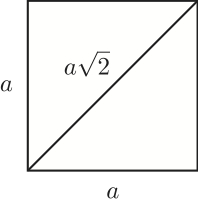
\includegraphics{square.png}
\end{center}
\vspace{-.5cm}
\caption{The side and diagonal of a square are incommensurable.}
\label{fig:square}
\end{figure}

Before tackling a proof of Theorem~\ref{thm:sqrt2}, we need a few tools.  In particular, we will make use of the Fundamental Theorem of Arithmetic (see Corollary~\ref{cor:FTA}).  The following result makes up half of the Fundamental Theorem of Arithmetic.

\begin{theorem}[*]\label{thm:prodprimes}
Let $n$ be a natural number greater than 1.  Then $n$ can be expressed as a product of primes.  That is, we can write
\[
n=p_1 p_2 \cdots p_k,
\]
where each of $p_1, p_2, \ldots, p_k$ are prime numbers (and there may possibly be repeats in this list).\footnote{\emph{Hint:} Use a proof by contradiction.  Let $n$ be the smallest natural number for which the theorem fails.  Then $n$ cannot be prime since this would satisfy the theorem.  So, it must be the case that $n$ has a divisor other than 1 and itself.  This implies that there exists natural numbers $a$ and $b$ greater than 1 such that $n=ab$.  Since $n$ was our smallest counterexample, what can you conclude about both $a$ and $b$?  Use this information to derive a counterexample for $n$.}
\end{theorem}

The previous theorem states that we can write every natural number as a product of primes, but it does not say that the primes and the number of times the primes appear are unique.  It turns out that this is fairly difficult to prove.  We will need the following result known as the Division Algorithm, but we won't worry about proving it.  Instead, we will take it for granted and use it in the proof of Theorem~\ref{thm:Euclid}, which we will then use to prove uniqueness.

\begin{theorem-given}[Division Algorithm]
Suppose that $m,n\in\mathbb{N}$.  Then there exists unique $q,r\in\mathbb{N}$ such that $m=nq+r$ with $0\leq r<n$.
\end{theorem-given}
The numbers $q$ and $r$ from the Division Algorithm are referred to as \textbf{quotient} and \textbf{remainder}, respectively.  Now, see if you can prove the following theorem, which is known as Euclid's Lemma.

\begin{theorem}[Euclid's Lemma, *]\label{thm:Euclid}
Assume that $p$ is prime.  If $p$ divides $ab$, where $a,b\in\mathbb{N}$, then either $p$ divides $a$ or $p$ divides $b$.\footnote{\emph{Hint:} Use a proof by contradiction and apply the Division Algorithm to both $a$ and $b$.  What can you say about $ab$?}
\end{theorem}

Alright, let's tackle the uniqueness of the product of primes now.

\begin{theorem}[*]\label{thm:unique}
Let $n$ be a natural number greater than 1.  Then the expression for $n$ as the product of one or more primes is unique (up to the order in which they appear).\footnote{\emph{Hint:} Use a proof by contradiction.  Write $n$ as both $p_1 p_2 \cdots p_k$ and $q_1 q_2 \cdots q_l$, where both are products of primes.  Use Euclid's Lemma to derive a contradiction.}
\end{theorem}

The following corollary follows immediately from Theorem~\ref{thm:prodprimes} and Theorem~\ref{thm:unique}.

\begin{corollary}[Fundamental Theorem of Arithmetic]\label{cor:FTA}
Every natural number greater than 1 can be expressed uniquely (up to the order in which they appear) as the product of one or more primes.
\end{corollary}

We are finally ready to prove that $\sqrt{2}$ is irrational.

\begin{theorem}[*]
\label{thm:sqrt2}
The real number $\sqrt{2}$ is irrational.\footnote{\emph{Hint:} Use a proof by contradiction.  That is, suppose that there exist $m,n\in\mathbb{Z}$ such that $n\ne 0$ and $\sqrt{2}=\frac{m}{n}$. Next, square both sides and solve for $m^2$. How many factors of 2 does $m^2$ have?  How many factors of 2 does $2n^2$ have? Derive a contradiction using Corollary~\ref{cor:FTA}.}
\end{theorem}

As one might expect, the Pythagoreans were unhappy with this discovery. Legend says that Hippasus was expelled from the Pythagoreans and was perhaps drowned at sea. Ironically, this result, which angered the Pythagoreans so much, is probably their greatest contribution to mathematics: the discovery of irrational numbers.

Now, let's tackle a few more problems dealing with irrational numbers.

\begin{problem}
Determine whether $\displaystyle \frac{1+\sqrt{2}}{3+2\sqrt{2}}$ is rational or irrational and then prove that your answer is correct.
\end{problem}

\begin{theorem}[*]\label{thm:sqrtp}
Let $p$ be a prime number.  Then $\sqrt{p}$ is irrational.
\end{theorem}

\begin{exercise}
Let $p$ be a prime number.  For which values of $n\in\mathbb{N}$ is $\sqrt[n]{p}$ irrational?  You do not need to prove your answer.
\end{exercise}

\begin{theorem}[*]\label{thm:sqrt(pq)}
Let $p$ and $q$ be distinct primes.  Then $\sqrt{pq}$ is irrational.
\end{theorem}

\begin{problem}
State a generalization of Theorem~\ref{thm:sqrt(pq)} and briefly describe how its proof would go.  Be as general as possible.
\end{problem}

\begin{remark}
It is important to point out that not every positive irrational number is equal to the square root of some natural number.  For example, $\pi$ is irrational, but is not equal to the square root of a natural number.
\end{remark}

It is worth pointing out that our approach for proving that $\sqrt{2}$ was irrational was not the most efficient.  However, our technique was easy to generalize to handle results like Theorem~\ref{thm:sqrtp}.

\end{section}

%%% Local Variables: 
%%% mode: latex
%%% TeX-master: "IntroToProof"
%%% End: 

\clearpage\begin{section}{The infinitude of primes}

The highlight of this section\footnote{This section is derived from work of \href{http://users.dickinson.edu/~richesod/}{Dave Richeson} of Dickinson College.} is Theorem~\ref{thm:infprimes}, which states that there are infinitely many primes. In case you forgot, here is the definition of a prime number.

\begin{definition}
A natural number $p$ is called \textbf{prime} iff $p$ is divisible by exactly two distinct natural numbers (namely, 1 and $p$ itself).
\end{definition}

\begin{exercise}
Is 1 a prime number?  Explain your answer.
\end{exercise}

The first known proof of Theorem~\ref{thm:infprimes} is in Eulcid's \emph{Elements} (c.\ 300 BCE). Euclid stated it as follows: 
\begin{quote}
\textbf{Proposition IX.20.} Prime numbers are more than any assigned multitude of prime numbers.
\end{quote}
There are a few interesting observations to make about Euclid's proposition and his proof. First, notice that the statement of the theorem does not contain the word ``infinity.'' The Greek's were skittish about the idea of infinity. Thus he proved that there were more primes than any given finite number. Today we'd say that they are infinite. In fact, Euclid proved that there are more than \emph{three} primes and concluded that there were more than any finite number. While you would lose points for such a proof in this class, we can forgive Euclid for this less-than-rigorous proof;  in fact, it is easy to turn his proof into the general one that you will give below. Lastly, Euclid's proof was geometric. He was viewing his numbers as line segments with integral length. The modern concept of number was not developed yet.

Prior to tackling a proof of Theorem~\ref{thm:infprimes}, we need to prove a couple lemmas.  The proof of the first lemma is provided for you. 

\begin{lemma-given}\label{lem:divisorsof1}
The only natural number that divides $1$ is $1$.  
\end{lemma-given}

\begin{proof}
Let $m$ be a natural number that divides $1$. We know that $m\geq 1$ because 1 is the smallest positive integer. Since $m$ divides $1$, there exists $k\in \mathbb{N}$ such that $1=mk$. Since $k\geq 1$, we see that $mk\geq m$.  But $1=mk$, and so $1\geq m$.  Thus, we have $1\leq m \leq 1$, which implies that $m=1$, as desired.
\end{proof}

\begin{lemma}\label{lem:plus1}
Let $p$ be a prime number  and let $n\in \mathbb{Z}$. If $p$ divides $n$, then $p$ does not divide $n+1$.\footnote{\emph{Hint:} Use a proof by contradiction and utilize the previous lemma.}
\end{lemma}

Now, we are ready to prove the following important theorem.

\begin{theorem}\label{thm:infprimes}
There are infinitely many prime numbers.\footnote{\emph{Hint:} Use a proof by contradiction.  In this case, there are finitely many primes.  Consider the product of all of them and then add 1.}
\end{theorem}

\end{section}



%%% Local Variables: 
%%% mode: latex
%%% TeX-master: "IntroToProof"
%%% End: 




% Relations and functions
\chapter{Relations and Functions}

\begin{section}{Relations}

\begin{definition}
An \textbf{ordered pair} is an object of the form $(x,y)$. Two ordered pairs $(x,y)$ and $(a,b)$ are \textbf{equal} if $x=a$ and $y=b$. 
\end{definition}

\begin{definition}
An \textbf{$n$-tuple} is an object of the form $(x_1, x_2,\ldots,x_n)$.  Each $x_i$ is referred to as the $i$th \textbf{component}.
\end{definition}

Note that an ordered pair is just a 2-tuple.

\begin{definition}
If $X$ and $Y$ are sets, the \textbf{Cartesian product} of $X$ and $Y$ is defined by
\[
X\times Y=\{(x,y): x\in X, y\in Y\}.
\]
That is, $X\times Y$ is the set of all ordered pairs where the first element is from $X$ and the second element is from $Y$.  The set $X\times X$ is sometimes denoted by $X^2$.  We similarly define the Cartesian product of $n$ sets, say $X_1, \ldots, X_n$, by
\[
\prod_{i=1}^{n} X_i=X_1\times \cdots \times X_n=\{(x_1,\ldots,x_n): \mbox{each } x_i\in X_i\}.
\]
\end{definition}

\begin{example}
Let $A=\{a,b,c\}$ and $B=\{\smiley,\frownie\}$.  Then 
\[
A\times B=\{(a,\smiley), (a,\frownie),(b,\smiley),(b,\frownie), (c,\smiley),(c,\frownie)\}.
\]
\end{example}

\begin{exercise}
Using the sets $A$ and $B$ from the previous example, find $B\times A$.  
\end{exercise}

\begin{exercise}
Using the set $B$ from the previous examples, find $B\times B$.  
\end{exercise}

\begin{exercise}
What general conclusion can you make about $X\times Y$ versus $Y\times X$?  When will they be equal?
\end{exercise}

\begin{exercise}
If $X$ and $Y$ are both finite sets, then how many elements will $X\times Y$ have?  Be as specific as possible.
\end{exercise}

\begin{exercise} 
Let $A=\{1, 2, 3\}$, $B=\{1,2\}$, and $C=\{1,3\}$. List the elements of the set $A \times B\times C$. 
\end{exercise}

\begin{exercise}
Let $A=\mathbb{N}$ and $B=\mathbb{R}$. Describe the elements of the set $A \times B$. 
\end{exercise}

\begin{exercise} Let $A$ be the set of all differentiable functions on the open interval $(0,1)$, and let $B$ equal the set of all derivatives of functions in $A$ evaluated at $x=\frac{1}{2}$. Describe the elements of the set $A \times B$. \end{exercise}

\begin{exercise}
Three space, $\mathbb{R}^{3}$, is a Cartesian product.  Unpack the meaning of $\mathbb{R}^{3}$ using the Cartesian product, and write the complete set notation version.
\end{exercise}

\begin{exercise}
Let $X=[0,1]$ and let $Y=\{1\}$.  Describe geometrically what $X\times Y$, $Y\times X$, $X\times X$, and $Y\times Y$ look like.
\end{exercise}

\begin{definition}
Let $X$ and $Y$ be sets. A \textbf{relation} from a set $X$ to a set $Y$ is a subset of $X \times Y$. A relation on $X$ is a subset of $X \times X$.  
\end{definition}

\begin{example}
You may not realize it, but you are familiar with many relations.  For example, on the real numbers, we have the relation $\leq$.  We could say that $(3,\pi)$ is in the relation since $3\leq \pi$.  However, $(1,-1)$ is not in the relation since $1\nleq -1$.  (Order matters!)
\end{example}

\begin{remark}
Different notations for relations are used in different contexts.  When talking about relations in the abstract, we indicate that a pair $(a,b)$ is in the relation by some notation like $a\sim b$, which is read ``$a$ is related to $b$."
\end{remark}

\begin{example}
Let $P_f$ denote the set of all people with accounts on Facebook.  Define  $F$ via $xFy$ iff $x$ is friends with $y$.  Then $F$ is a relation on $P_f$.
\end{example}

\begin{remark}
We can often represent relations using graphs or digraphs.  Given a finite set $X$ and a relation $\sim$ on $X$, a \textbf{digraph} (short for \emph{directed graph}) is a discrete graph having the members of $X$ as vertices and a directed edge from $x$ to $y$ iff $x\sim y$.
\end{remark}

\begin{example}
Figure~\ref{fig:digraph} depicts a digraph that represents a relation $R$ given by
\[
R=\{(a,b),(a,c),(b,b),(b,c),(c,d),(c,e),(d,d),(d,a),(e,a)\}.
\]

\begin{figure}[h]
\begin{center}
\begin{tikzpicture}[->,>=stealth',shorten >=1pt,auto,node distance=2cm,
                    semithick]
  \tikzstyle{every state}=[]

  \node[state] (A)                    {$a$};
  \node[state]         (B) [above right of=A] {$b$};
  \node[state]         (D) [below right of=A] {$d$};
  \node[state]         (C) [below right of=B] {$c$};
  \node[state]         (E) [below of=D]       {$e$};

  \path (A) edge              node {} (B)
            edge              node {} (C)
        (B) edge [loop above] node {} (B)
            edge              node {} (C)
        (C) edge              node {} (D)
            edge [bend left]  node {} (E)
        (D) edge [loop below] node {} (D)
            edge              node {} (A)
        (E) edge [bend left]  node {} (A);
\end{tikzpicture}
\caption{An example of a digraph for a relation.}\label{fig:digraph}
\end{center}
\end{figure}


\end{example}

\begin{exercise}
Let $A=\{a,b,c\}$ and define $\sim=\{(a,a),(a,b),(b,c),(c,b),(c,a)\}$.  Draw the digraph for $\sim$.
\end{exercise}

\begin{exercise}
Let $A=\{1,2,3,4,5,6\}$.  Define $|$ on $A$ via $x|y$ iff $x$ divides $y$.  Draw the digraph for $|$ on $A$.
\end{exercise}

When $X$ or $Y$ is infinite, it is not practical to draw a digraph.  However, you are familiar with the graphs of some relations involving infinite sets.

\begin{example}
When we write $x^2+y^2=1$, we are implicitly defining a relation.  In particular, the relation is the set of ordered pairs $(x,y)$ satisfying $x^2+y^2=1$.  In set notation:
\[
\{(x,y):x^2+y^2=1\}
\]
The graph of this relation in $\mathbb{R}^2$ is the standard unit circle.
\end{example}

\begin{exercise}
Define $\sim$ on $\mathbb{R}$ via $x\sim y$ iff $x\leq y$.  Draw a
picture of this relation in $\mathbb{R}^2$ (in other words, draw all
points $(x,y)$ where $x\sim y$).
\end{exercise}

\begin{definition}
Let $\sim$ be a relation on a set $A$.
\begin{enumerate}
\item $\sim$ is \textbf{reflexive} if for all $x\in A$, $x\sim x$ (every element is related to itself).
\item $\sim$ is \textbf{symmetric} if for all $x,y\in A$, if $x\sim y$, then $y\sim x$.
\item $\sim$ is \textbf{transitive} if for all $x,y,z\in A$, if $x\sim y$ and $y\sim z$, then $x\sim z$.
\end{enumerate}
\end{definition}

\begin{example}\
\begin{enumerate}
\item $\leq$ on $\mathbb{R}$ is reflexive and transitive, but not symmetric.
$<$ on $\mathbb{R}$ is transitive, but not symmetric and not reflexive.
\item If $S$ is a set, then $\subseteq$ on $\mathcal{P}(S)$ is reflexive and transitive, but not symmetric.
\item $=$ on $\mathbb{R}$ is reflexive, symmetric, and transitive.
\end{enumerate}

\end{example}

\begin{exercise}
Given a finite set $A$ and a relation $\sim$, describe what each of reflexive, symmetric, and transitive look like in terms of a digraph.
\end{exercise}

\begin{exercise}
Let $P$ be the set of people at a party and define $N$ via $(x,y)\in N$ iff $x$ knows the name of $y$.  Describe what it would mean for $N$ to be reflexive, symmetric, and transitive.
\end{exercise}

\begin{exercise}
Determine whether each of the following relations is reflexive, symmetric, or transitive.

\begin{enumerate}
\item Let $P_f$ denote the set of all people with accounts on Facebook.  Define  $F$ via $xFy$ iff $x$ is friends with $y$. 
\item Let $P$ be the set of all people and define $H$ via $xHy$ iff $x$ and $y$ have the same height.
\item Let $P$ be the set of all people and define $T$ via $xTy$ iff $x$ is taller than $y$.
\item Consider the relation ``divides" on $\mathbb{N}$.
\item Let $L$ be the set of lines and define $||$ via $l_1||l_2$ iff $l_1$ is parallel to $l_2$.
\item Let $C[0,1]$ be the set of continuous functions on $[0,1]$.  Define $f\sim g$ iff
\[
\int_0^1|f(x)|\ dx=\int_0^1|g(x)|\ dx.
\]
\item Define $\sim$ on $\mathbb{N}$ via $n\sim m$ iff $n+m$ is even.
\item Define $D$ on $\mathbb{R}$ via $(x,y)\in D$ iff $x=2y$.
\end{enumerate}
\end{exercise}


\end{section}


%%% Local Variables: 
%%% mode: latex
%%% TeX-master: "IntroToProof"
%%% End: 

\clearpage\begin{section}{Equivalence Relations}

\begin{remark}
So that we have them handy, let's recall the following definitions. Let $\sim$ be a relation on a set $A$.  Then
\begin{enumerate}
\item $\sim$ is \textbf{reflexive} if for all $x\in A$, $x\sim x$ (every element is related to itself).
\item $\sim$ is \textbf{symmetric} if for all $x,y\in A$, if $x\sim y$, then $y\sim x$.
\item $\sim$ is \textbf{transitive} if for all $x,y,z\in A$, if $x\sim y$ and $y\sim z$, then $x\sim z$.
\end{enumerate}
As we've seen in the previous section of notes, these conditions are mutually exclusive.  That is, a relation may have some combination of these properties, but not necessarily all of them.  However, we have a special name for when a relation does satisfy all three.
\end{remark}

\begin{definition}
Let $\sim$ be a relation on a set $A$.  Then $\sim$ is called an \textbf{equivalence relation} if $\sim$ is reflexive, symmetric, and transitive.
\end{definition}

\begin{exercise}
Given a finite set $A$ and a relation $\sim$ on $A$, describe what the corresponding digraph would have to look like in order for $\sim$ to be an equivalence relation.
\end{exercise}

\begin{exercise}\label{exer:made up}
Let $A=\{a,b,c,d,e\}$.  Make up an equivalence relation on $A$ by drawing a digraph such that $a$ is not related to $b$ and $c$ is not related to $b$.
\end{exercise}

\begin{exercise}\label{exer:digraph}
Let $S=\{1,2,3,4,5,6\}$ and define
\[
\sim=\{(1,1),(1,6),(2,2),(2,3),(2,4),(3,3),(3,2),(3,4),(4,4),(4,2),(4,3),(5,5),(6,6),(6,1)\}.
\]
Justify that this is an equivalence relation.
\end{exercise}

\begin{problem}
Determine which of the following are equivalence relations.  Some of these occurred in the last section of notes and you are welcome to use your answers from those problems.

\begin{enumerate}\label{exer:lots of them}
\item\label{exer:facebook} Let $P_f$ denote the set of all people with accounts on Facebook.  Define  $F$ via $xFy$ iff $x$ is friends with $y$. 
\item Let $P$ be the set of all people and define $H$ via $xHy$ iff $x$ and $y$ have the same height.
\item Let $P$ be the set of all people and define $T$ via $xTy$ iff $x$ is taller than $y$.
\item Consider the relation ``divides" on $\mathbb{N}$.
\item Let $L$ be the set of lines and define $||$ via $l_1||l_2$ iff $l_1$ is parallel to $l_2$.
\item Let $C[0,1]$ be the set of continuous functions on $[0,1]$.  Define $f\sim g$ iff
\[
\int_0^1|f(x)|\ dx=\int_0^1|g(x)|\ dx.
\]
\item Define $\sim$ on $\mathbb{N}$ via $n\sim m$ iff $n+m$ is even.
\item Define $D$ on $\mathbb{R}$ via $(x,y)\in D$ iff $x=2y$.
\item\label{exer:mod 5} Define $\sim$ on $\mathbb{Z}$ via $a\sim b$ iff $a-b$ is a multiple of 5.
\item Define $\sim$ on $\mathbb{R}^2$ via $(x_1,y_1)\sim (x_2,y_2)$ iff $x_1^2+y_1^2=x_2^2+y_2^2$.
\item Define $\sim$ on $\mathbb{R}$ via $x\sim y$ iff $\lfloor x\rfloor =\lfloor y\rfloor$, where $\lfloor x\rfloor$ is the greatest integer less than or equal to $x$ (e.g., $\lfloor \pi\rfloor=3$, $\lfloor -1.5\rfloor=-2$, and $\lfloor 4\rfloor=4$).
\item Define $\sim$ on $\mathbb{R}$ via $x \sim y$ iff $|x-y|<1$.
\end{enumerate}
\end{problem}

\begin{definition}
Let $\sim$ be a relation on a set $A$ (not necessarily an equivalence relation) and let $x\in A$.  Then we define the \textbf{set of relatives of $x$} via
\[
[x]=\{y\in A: x\sim y\}.
\]
Also, define
\[
\Omega_{\sim}=\{[x]:x\in A\}.
\]
Notice that $\Omega_{\sim}$ is a set of sets.  In particular, an element in $\Omega_{\sim}$ is a subset of $A$ (equivalently, an element of $\mathcal{P}(A)$).  Other common notations for $[x]$ include $\overline{x}$ and $R_x$.
\end{definition}

\begin{exercise}
Let $P_f$ and $F$ be as in part \ref{exer:facebook} of Exercise \ref{exer:lots of them}.  Describe $[\text{Bob}]$ (assume you know which Bob we're talking about).  What is $\Omega_F$?
\end{exercise}

\begin{exercise}
Using your digraph in Exercise \ref{exer:made up}, find $\Omega_{\sim}$ for all $x\in A$.  
\end{exercise}

\begin{exercise}
Consider the relation $\leq$ on $\mathbb{R}$.  If $x\in \mathbb{R}$, what is $[x]$?
\end{exercise}

\begin{exercise}
Find $[1]$ and $[2]$ for the relation given in part \ref{exer:mod 5} of Exercise \ref{exer:lots of them}.  How many different sets of relatives are there?  What are they?
\end{exercise}

\begin{exercise}
Find $[x]$ for all $x\in S$ for $S$ and $\sim$ from Exercise \ref{exer:digraph}.  Any observations?
\end{exercise}

\begin{theorem}[*]\label{thm:equiv same class}
Suppose $\sim$ is an equivalence relation on a set $A$ and let $a,b\in A$.  Then $[a]=[b]$ iff $a\sim b$.
\end{theorem}

\begin{theorem}[*]\label{thm:equiv yields partition}
Suppose $\sim$ is an equivalence relation on a set $A$.  Then
\begin{enumerate}
\item $\bigcup_{x\in A}[x]=A$, and
\item for all $x,y\in A$, either $[x]=[y]$ or $[x]\cap [y]=\emptyset$.
\end{enumerate}
\end{theorem}

\begin{definition}
In light of Theorem \ref{thm:equiv yields partition}, if $\sim$ is an equivalence relation on a set $A$, then we refer to each $[x]$ as the \textbf{equivalence class} of $x$.  In this case, $\Omega_{\sim}$ is the set of equivalence classes determined by $\sim$.
\end{definition}

\begin{remark}
The upshot of Theorem \ref{thm:equiv yields partition} is that given an equivalence relation, every element lives in exactly one equivalence class.  We'll see in the next section of notes that we can run this in reverse.  That is, if we separate out the elements of a set so that every element is an element of exactly one subset (like the bins of my kid's toys), then this determines an equivalence relation.  More on this later.
\end{remark}

\begin{example}
The set of relatives that you found in part \ref{exer:mod 5} of Exercise \ref{exer:lots of them} is the set of equivalence classes modulo 5.
\end{example}

\begin{exercise}
If $\sim$ is an equivalence relation on a finite set $A$, then what is the connection between the equivalence classes and the corresponding digraph?
\end{exercise}

\begin{exercise}
For each of the equivalence relations in Exercise \ref{exer:lots of them}, describe the equivalence classes as best as you can.
\end{exercise}

\end{section}


%%% Local Variables: 
%%% mode: latex
%%% TeX-master: "IntroToProof"
%%% End: 

\clearpage\begin{section}{Partitions}

\begin{remark}
The upshot of Theorems~\ref{thm:equiv same class} and \ref{thm:equiv
  yields partition} is that if $\sim$ is an equivalence relation on a set $A$, then $\sim$ breaks $A$ up into pairwise disjoint chunks, where each chunk is some $[a]$ for $a\in A$. Furthermore, each  pair of elements in the same set of relatives are related via $\sim$.
\end{remark}

As you've probably already noticed, equivalence relations are intimately related to the following concept.

\begin{definition}
A collection $\Omega$ of nonempty subsets of a set $A$ is said to be a \textbf{partition} of $A$ if the elements of $\Omega$ satisfy:
\begin{enumerate}
\item Given $X,Y\in\Omega$, either $X=Y$ or $X\cap Y=\emptyset$ (We can't have both at the same time. Do you see why?), and
\item $\displaystyle \bigcup_{X\in\Omega}X=A$.
\end{enumerate}
That is, the elements of $\Omega$ are pairwise disjoint and their union is all of $A$.
\end{definition}

\begin{example}
The following are all examples of partitions of the given set.  Perhaps you can find exceptions in these examples, but please take them at face value.
\begin{enumerate}
\item men, women (set of people)
\item Democrat, Republican, Independent, Green Party, Libertarian, etc. (set of registered voters)
\item freshman, sophomore, junior, senior (set of high school students)
\item evens, odds (set of integers)
\item rationals, irrationals (set of real numbers)
\end{enumerate}
\end{example}

\begin{example}\label{ex:a partition}
Let $A=\{a,b,c,d,e,f\}$ and $\Omega=\{X_{1},X_{2},X_{3}\}$, where $X_{1}=\{a\}$, $X_{2}=\{b,c,d\}$, and $X_{3}=\{e,f\}$.  Then $\Omega$ is a partition of $A$ since the elements of $\Omega$ are pairwise disjoint and their union is all of $A$.
\end{example}

\begin{exercise}
Consider the set $A$ from Example \ref{ex:a partition}.
\begin{enumerate}
\item Find a partition of $A$ that has 4 subsets in the partition.
\item Find a collection of subsets of $A$ that does \emph{not} form a partition.
\end{enumerate}
\end{exercise}

\begin{exercise}
Find a partition of $\mathbb{N}$ that consists of 3 subsets, where one of the sets is finite and the remaining two sets are infinite.
\end{exercise}

\begin{exercise}
Let $P$ be the set of prime numbers, $N$ be the set of odd natural numbers that are not prime, and $E$ be the set of even natural numbers.  Explain why this is not a partition of $\mathbb{N}$.
\end{exercise}

The next theorem spells out half of the close connection between partitions and equivalence relations.  Hopefully you were anticipating this.

\begin{theorem}[*]
Let $\sim$ be an equivalence relation on a set $A$.  Then $\Omega_{\sim}$ forms a partition of $A$.
\end{theorem}

\begin{exercise}
Consider the equivalence relation
\[
\sim=\{(1,1),(1,2),(2,1), (2,2),(3,3),(4,4),(4,5),(5,4),(5,5),(6,6),(5,6),(6,5),(4,6),(6,4)\}
\]
on the set $A=\{1,2,3,4,5,6\}$.  Find the partition determined by $\Omega_{\sim}$.
\end{exercise}

It turns out that we can reverse the situation, as well.  That is, given a partition, we can form an equivalence relation.  Before proving this, we need a definition.

\begin{definition}
Let $A$ be a set and $\Omega$ any collection of subsets from $\mathcal{P}(A)$ (not necessarily a partition).  If $a,b\in A$, we will define $a$ to be $\Omega$-related to $b$ if there exists an $R\in \Omega$ that contains both $a$ and $b$.  This relation is denoted by $\sim_{\Omega}$ and is called the \textbf{relation on $A$ associated to $\Omega$}.
\end{definition}

\begin{remark}
This definition may look more awkward than the actual underlying concept.  The idea is that if two elements are in the same subset, then they are related.  For example, when my kids pick up all their toys and put them in the appropriate toy bins, we say that two toys are related if they are in the same bin.
\end{remark}

\begin{remark}
Notice that we have two notations that looks similar: $\Omega_{\sim}$ and $\sim_{\Omega}$.  
\begin{enumerate}
\item $\Omega_{\sim}$ is the collection of subsets of $A$ determined by the relation $\sim$.
\item $\sim_{\Omega}$ is the relation determined by the collection of subsets $\Omega$.
\end{enumerate}
\end{remark}

\begin{exercise}
Let $A=\{a,b,c,d,e,f\}$ and let $\Omega=\{X_{1},X_{2},X_{3}\}$, where $X_{1}=\{a,c\}$, $X_{2}=\{b,c\}$, and $X_{3}=\{d,f\}$.  List the elements of $\sim_{\Omega}$ by listing ordered pairs or drawing a digraph.
\end{exercise}

\begin{exercise}
Let $A$ and $\Omega$ be as in Example \ref{ex:a partition}.  List the elements of $\sim_{\Omega}$ by listing ordered pairs or drawing a digraph.
\end{exercise}

\begin{theorem}[*]
Let $A$ be a set and let $\Omega$ be a collection of subsets from $\mathcal{P}(A)$ (not necessarily a partition).  Then $\sim_{\Omega}$ is symmetric.
\end{theorem}

\begin{exercise}
Give an example of a set $A$ and a collection $\Omega$ from $\mathcal{P}(A)$ such that the relation $\sim_{\Omega}$ is not reflexive.
\end{exercise}

\begin{theorem}[*]
Let $A$ be a set and let $\Omega$ be a collection of subsets from $\mathcal{P}(A)$.  If $\displaystyle \bigcup_{R\in\Omega}R=A$, then $\sim_{\Omega}$ is reflexive.
\end{theorem}

\begin{theorem}[*]
Let $A$ be a set and let $\Omega$ be a collection of subsets from $\mathcal{P}(A)$.  If the elements of $\Omega$ are pairwise disjoint, then $\sim_{\Omega}$ is transitive.
\end{theorem}

\begin{corollary}[*]
Let $A$ be a set and let $\Omega$ be a partition of $A$.  Then $\sim_{\Omega}$ is an equivalence relation.
\end{corollary}

\begin{remark}
The previous corollary says that every partition determines a natural equivalence relation.  Namely, two elements are related if they are in the same equivalence class.
\end{remark}

\begin{exercise}
Let $A=\{\circ, \triangle, \blacktriangle, \square, \blacksquare, \bigstar, \smiley, \frownie\}$.  Make up a partition $\Omega$ on $A$ and then draw the digraph corresponding to $\sim_{\Omega}$.
\end{exercise}

\end{section}

%%% Local Variables: 
%%% mode: latex
%%% TeX-master: "IntroToProof"
%%% End: 

\clearpage\begin{section}{Introduction to Functions}

The concept of function is one of the most important and fundamental ones in the field of mathematics.  Functions are used in all branches of mathematics to model diverse situations and pull together ideas that at first seem unrelated.  Functions are as vital as numbers.

Undoubtably, you have encountered the concept of function in your prior mathematical experience.  In this section, we will introduce the concept of function as a special type of relation.  As you shall see, this agrees with any previous definition of function that you may have learned.  

Up until this point, you've probably only encountered functions as an algebraic rule, e.g. $f(x)=x^{2}-1$, for transforming one real number into another.  However, we can study functions in a much broader context.  Loosely speaking, the basic building blocks of a function are a first set and a second sets, say $X$ and $Y$, respectively, and a ``correspondence'' that assigns to each element of $X$ to exactly one element of $Y$.  Let's take a look at the actual definition.

\begin{definition}
Let $X$ and $Y$ be two nonempty sets.  A \textbf{function} from set $X$ to set $Y$, denoted $f:X\to Y$, is a relation (i.e., subset of $X\times Y$) such that:

\begin{enumerate}\label{def:function}
\item For each $x\in X$, there exists $y\in Y$ such that $(x,y)\in f$, and
\item If $(x,y_{1}), (x,y_{2}) \in f$, then $y_{1}=y_{2}$.
\end{enumerate}
Note that if $(x,y)\in f$, we usually write $y=f(x)$ and say that ``$f$ maps $x$ to $y$.''
\end{definition}

\begin{remark}
Item 1 of Definition \ref{def:function} says that every element of $X$ appears in the first coordinate of an ordered pair in the relation.  Item 2 says that each element of $X$ only appears once in the first coordinate of an ordered pair in the relation.  It is important to note that there are no restrictions on whether an element of $Y$ ever appears in the second coordinate.  Furthermore, if an element of $B$ appears in the second coordinate, it may appear again in a different ordered pair.
\end{remark}

\begin{definition}
The set $X$ from Definition \ref{def:function} is called the \textbf{domain} of $f$ and is denoted by $\dom(f)$.  The set $Y$ is called the \textbf{codomain} of $f$ and is denoted by $\codom(f)$.  The set
\[
\range(f)=\{y\in Y: \mbox{there exists }x\mbox{ such that } y=f(x)\}
\]
is called the \textbf{range} of $f$ or the \textbf{image of $X$} under $f$.
\end{definition}

\begin{remark}
It follows immediately from the definition that $\range(f)\subseteq \codom(f)$.  However, it is possible that the range of $f$ is strictly smaller.
\end{remark}

\begin{remark}
If $f$ is a function and $(x,y)\in f$, then we may refer to $x$ as the \textbf{input} of $f$ and $y$ as the \textbf{output} of $f$.
\end{remark}

\begin{exercise}\label{exer:lots}
Let $X=\{\circ, \square,\triangle,\smiley\}$ and $Y=\{a,b,c,d,e\}$.  Determine whether each of the following represent functions.  Explain.  If the relation is a function, determine the domain, codomain, and range.

\begin{enumerate}
\item $f:X\to Y$ defined via $f=\{(\circ, a),(\square,b),(\triangle,c),(\smiley,d)\}$.
\item $g:X\to Y$ defined via $g=\{(\circ, a),(\square,b),(\triangle,c),(\smiley,c)\}$.
\item $h:X\to Y$ defined via $h=\{(\circ, a),(\square,b),(\triangle,c),(\circ,d)\}$.
\item $k:X\to Y$ defined via $k=\{(\circ, a),(\square,b),(\triangle,c),(\smiley,d),(\square,e)\}$.
\item $l:X\to Y$ defined via $l=\{(\circ, e),(\square,e),(\triangle,e),(\smiley,e)\}$.
\item $m:X\to Y$ defined via $m=\{(\circ, a),(\triangle,b),(\smiley,c)\}$.
\item $\operatorname{happy}:Y\to X$ defined via $\operatorname{happy}(y)=\smiley$ for all $y\in Y$.
\item $\operatorname{id}:X\to X$ defined via $\operatorname{id}(x)=x$ for all $x\in X$.
\item $\operatorname{nugget}:X\to X$ defined via 
\[
\operatorname{nugget}(x)=\begin{cases}
x, & \mbox{if } x\mbox{ is a geometric shape},\\
\square, & \mbox{otherwise}.
\end{cases}
\]
\end{enumerate}
\end{exercise}

\begin{definition}
One useful representation of functions on finite sets is via \textbf{bubble diagrams}.  To draw a bubble diagram for a function $f:X\to Y$, draw one circle (i.e, a ``bubble'') for each of $X$ and $Y$ and for each element of each set, put a dot in the corresponding set.  Typically, we draw $X$ on the left and $Y$ on the right.  Now, draw an arrow from $x\in X$ to $y\in Y$ if $f(x)=y$ (i.e., $(x,y)\in f$).  In fact, we can draw bubble diagrams even if $f$ isn't a function.
\end{definition}

\begin{exercise}
For each of the relations in Exercise \ref{exer:lots} draw the corresponding bubble diagram.
\end{exercise}

\begin{problem}
What properties does a bubble diagram have to have in order to represent a function?
\end{problem}

\begin{exercise}
Provide an example of each of the following.  You may draw a bubble diagram, write down a list of ordered pairs, or a write a formula (as long as the domain and codomain are clear).
\begin{enumerate}
\item A function $f$ from a set with 4 elements to a set with 3 elements such that $\range(f)=\codom(f)$.
\item A function $g$ from a set with 4 elements to a set with 3 elements such that $\range(g)$ is strictly smaller than $\codom(g)$.
\end{enumerate}
\end{exercise}

\begin{problem}
Let $f:X\to Y$ be a function and suppose that $X$ and $Y$ have $n$ and $m$ elements in them, respectively.  Also, suppose that $n<m$.  Is it possible for $\range(f)=\codom(f)$?  Explain.
\end{problem}

\begin{problem}
In high school I am sure that you were told that a graph represents a function if it passes the \textbf{vertical line test}.  Using our terminology of ordered pairs, explain why this works.
\end{problem}

\begin{definition}
Two functions are equal if they have the same domain, same codomain, and the same set of ordered pairs in the relation.
\end{definition}

\begin{remark}
If two functions are defined by the same algebraic formula, but have different domains, then they are \emph{not} equal.  For example, the function $f:\mathbb{R}\to \mathbb{R}$ defined via $f(x)=x^{2}$ is not equal to the function $g:\mathbb{N}\to\mathbb{N}$ defined via $g(x)=x^{2}$.
\end{remark}

\begin{theorem}
If $f:X\to Y$ and $g:X\to Y$ are functions, then $f=g$ iff $f(x)=g(x)$ for all $x\in X$.
\end{theorem}

\begin{definition}
Let $f:X\to Y$ be a function.
\begin{enumerate}
\item The function $f$ is said to be \textbf{one-to-one} (or \textbf{injective}) if for all $y\in \range(f)$, there is a unique $x\in X$ such that $y=f(x)$.
\item The function $f$ is said to be \textbf{onto} (or \textbf{surjective}) if for all $y\in Y$, there exists $x\in X$ such that $y=f(x)$.
\item If $f$ is both one-to-one and onto, we say that $f$ is a \textbf{one-to-one correspondence} (or a \textbf{bijection}).
\end{enumerate}
\end{definition}

\begin{exercise}
Provide an example of each of the following.  You may draw a bubble diagram, write down a list of ordered pairs, or write a formula (as long as the domain and codomain are clear).  Assume that $X$ and $Y$ are finite sets.
\begin{enumerate}
\item A function $f:X\to Y$ that is one-to-one but not onto.
\item A function $f:X\to Y$ that is onto but not one-to-one.
\item A function $f:X\to Y$ that is both one-to-one and onto.
\item A function $f:X\to Y$ that is neither one-to-one nor onto.
\end{enumerate}

\end{exercise}

\begin{problem}
Perhaps you've heard of the \textbf{horizontal line test} (i.e., every horizontal line hits the graph of $f:\mathbb{R}\to\mathbb{R}$ at most once).  What is the horizontal line test testing for?  Explain.
\end{problem}

\begin{exercise}
Provide an example of each of the following.  You may either draw a graph or write down a formula.  Make sure you have the correct domain.
\begin{enumerate}
\item A function $f:\mathbb{R}\to \mathbb{R}$ that is one-to-one but not onto.
\item A function $f:\mathbb{R}\to \mathbb{R}$ that is onto but not one-to-one.
\item A function $f:\mathbb{R}\to \mathbb{R}$ that is both one-to-one and onto.
\item A function $f:\mathbb{R}\to \mathbb{R}$ that is neither one-to-one nor onto.
\end{enumerate}

\end{exercise}

\begin{theorem}[*]
Let $f:X\to Y$ be a function.  Then $f$ is one-to-one iff for all $x_{1}, x_{2}\in X$, if $f(x_{1})=f(x_{2})$, then $x_{1}=x_{2}$.
\end{theorem}

\begin{remark}
The previous theorem gives a technique for proving that a given function is one-to-one.  Start by assuming that $f(x_{1})=f(x_{2})$ and then work to show that $x_{1}=x_{2}$.
\end{remark}

\begin{remark}
To show that a given function is onto, you should start with an arbitrary $y\in \range(f)$ and then work to show that there exists $x\in X$ such that $y=f(x)$.
\end{remark}

\begin{exercise}
Determine which of the following functions are one-to-one, onto, both, or neither.  In each case, you should provide proofs and counterexamples as appropriate.

\begin{enumerate}
\item $f:\mathbb{R}\to \mathbb{R}$ defined via $f(x)=x^{2}$
\item $g:\mathbb{R}\to [0,\infty)$ defined via $g(x)=x^{2}$
\item $h:\mathbb{R}\to \mathbb{R}$ defined via $h(x)=x^{3}$
\item $k:\mathbb{R}\to \mathbb{R}$ defined via $k(x)=x^{3}-x$
\item $l: \mathbb{R}\times \mathbb{R}\to \mathbb{R}$ defined via $l(x_{1},x_{2})=x_{1}^{2}+x_{2}^{2}$
\item $N:\mathbb{N}\to \mathbb{N}\times \mathbb{N}$ defined via $N(n)=(n,n)$
\end{enumerate}
\end{exercise}

\begin{exercise}
Let $A$ and $B$ be sets and let $S\subseteq A\times B$.  Define $\pi_{1}:S\to A$ and $\pi_{2}:S\to B$ via $\pi_{1}(a,b)=a$ and $\pi_{2}(a,b)=b$.  We call $\pi_{1}$ (respectively, $\pi_{2}$) the \textbf{projections} of $S$ onto $A$ (respectively, $B$).
\begin{enumerate}
\item Provide examples to show that $\pi_{1}$ does not need to be one-to-one or onto.
\item Suppose that $S$ is a function (recall that a function is a set of ordered pairs, so this makes sense).  Is $\pi_{1}$ one-to-one? Is $\pi_{1}$ onto?  How about $\pi_{2}$?
\end{enumerate} 
\end{exercise}

\end{section}


%%% Local Variables: 
%%% mode: latex
%%% TeX-master: "IntroToProof"
%%% End: 

\clearpage\begin{section}{Compositions and Inverses}

\begin{definition}
If $f:X\to Y$ and $g:Y\to Z$ are functions, then a new function $g\circ f:X\to Z$ can be defined by $(g\circ f)(x)=g(f(x))$ for all $x\in\dom(f)$.
\end{definition}

\begin{remark}
It is important to notice that the function on the right is the one that ``goes first.''
\end{remark}

\begin{exercise}
In each case, give examples of finite sets $X$, $Y$, and $Z$, and functions $f:X\to Y$ and $g:Y\to Z$ that satisfy the given conditions.  Drawing bubble diagrams is sufficient.
\begin{enumerate}
\item $f$ is onto, but $g\circ f$ is not onto.
\item $g$ is onto, but $g\circ f$ is not onto.
\item $f$ is one-to-one, but $g\circ f$ is not one-to-one.
\item $g$ is one-to-one, but $g\circ f$ is not.
\end{enumerate}
\end{exercise}

\begin{theorem}[*]
If $f:X\to Y$ and $g:Y\to Z$ are both functions that are onto, then $g\circ f$ is also onto.
\end{theorem}

\begin{theorem}[*]
If $f:X\to Y$ and $g:Y\to Z$ are both functions that are one-to-one, then $g\circ f$ is also one-to-one.
\end{theorem}

\begin{corollary}
If $f:X\to Y$ and $g:Y\to Z$ are both one-to-one correspondences, then $g\circ f$ is also a one-to-one correspondence.
\end{corollary}

\begin{problem}
Assume that $f:X\to Y$ and $g:Y\to Z$ are both functions.  For each of the following statements, if the statement is true, then prove it.  If the statement is false, provide a counterexample.
\begin{enumerate}
\item If $g\circ f$ is one-to-one, then $f$ is one-to-one.
\item If $g\circ f$ is one-to-one, then $g$ is one-to-one.
\item If $g\circ f$ is onto, then $f$ is onto.
\item If $g\circ f$ is onto, then $g$ is onto.
\end{enumerate}
\end{problem}

\begin{definition}
Let $f:X\to Y$ be a function.  The relation $f^{-1}$, called \textbf{$f$ inverse}, is defined via
\[
f^{-1}=\{(f(x),x):x\in X\}.
\]
\end{definition}

\begin{remark}
Notice that we called $f^{-1}$ a relation and not a function.  In some circumstances $f^{-1}$ will be a function and sometimes it won't be.
\end{remark}

\begin{exercise}
Provide an example of a function $f:X\to Y$ such that $f^{-1}$ is \emph{not} a function.  A bubble diagram is sufficient.
\end{exercise}

\begin{exercise}
Provide an example of a function $f:X\to Y$ such that $f^{-1}$ is a function. A bubble diagram is sufficient.
\end{exercise}

\begin{theorem}[*]
Let $f:X\to Y$ be a function.  Then $f^{-1}$ is a function iff $f$ is \underline{\ \ \ \ \ \ \ \ \ \ \ \ \ \ \ \ \ \ \ \ \ \ \ \ }.
\end{theorem}

\begin{theorem}[*]\label{thm:comp of inverses}
Let $f:X\to Y$ be a function and suppose that $f^{-1}$ is a function.  Then
\begin{enumerate}
\item $(f\circ f^{-1})(x)=x$ for all $x\in Y$, and
\item $(f^{-1}\circ f)(x)=x$ for all $x\in X$.
\end{enumerate}
(You only need to prove one of these statements; the other is similar.)
\end{theorem}

\begin{theorem}[*]\label{thm:unique inverse}
Let $f:X\to Y$ and $g:Y\to X$ be functions such that $f$ is a one-to-one correspondence.  If $(f\circ g)(x)=x$ for all $x\in Y$ and $(g\circ f)(x)=x$ for all $x\in X$, then $g=f^{-1}$.
\end{theorem}

\begin{remark}
The upshot of the previous two theorems is that if $f^{-1}$ is a function, then it is the only one satisfying the two-sided ``undoing'' property exhibited in Theorem \ref{thm:comp of inverses}.
\end{remark}

The next theorem can be considered to be a converse of Theorem \ref{thm:unique inverse}.

\begin{theorem}[*]
Let $f:X\to Y$ and $g:Y\to X$ be functions satisfying $(f\circ g)(x)=x$ for all $x\in Y$ and $(g\circ f)(x)=x$ for all $x\in X$.  Then $f$ is a one-to-one correspondence.
\end{theorem}

\begin{theorem}[*]
Let $f:X\to Y$ and $g:Y\to Z$ be functions.  If $f$ and $g$ are both one-to-one correspondences, then $(g\circ f)^{-1}=f^{-1}\circ g^{-1}$.
\end{theorem}

\end{section}

%%% Local Variables: 
%%% mode: latex
%%% TeX-master: "IntroToProof"
%%% End: 


\end{comment}

\end{document}

%%% Local Variables:
%%% mode: latex
%%% TeX-master: t
%%% End:
